\chapter{Setup Implementation}
\label{chap:implementation}

\section{Overview}

This work is focused in implementing a radio-frontend prototype for LTE band
communication and also has the task of documenting the whole process motivated
by the need of such device to act as a testbed for LTE band experimentations,
like algorithms or synchronization.

In this work, the Xilinx Vivado Suite was used to develop the FPGA design.
Intellectual properties were used through the IP integrator tool in the
Ultrafast design methodology \cite{xilinx:ultrafast}, which implement basic
functions or control peripherals of the FPGA board were also used to complement
the setup. Specific VHDL modules were developed to implement the integration
between transceiver and FPGA.

%----------------------------------FPGA-----------------------------------------
\section{FPGA}

FPGAs are digital integrated circuits (IC) that contain configurable
(programmable) blocks of logic along with configurable interconnects between
these blocks. Design engineers can configure (program) such devices to perform a
wide variety of tasks. Depending on the way in which they are built, some FPGA
boards may only be programmed a single time, like the Electronic programmable
read-only (EPROM) memory, while others may be reprogrammed over and over again,
which is the case of the FPGA boards used in this work \cite{max2004}.

The “field programmable” portion of the FPGA’s name refers to the fact that its
programming takes place “in the field” (as opposed to devices whose internal
functionality is hard-wired by the manufacturer). It means that FPGAs
connections are electrically activated and deactivated, thus the FPGA can be
programmed in a factory for large scale production or by the developer. When a
digital circuit, potentially designed by using FPGAs, is manufactured in a
self-contained hardwired integrated circuit, it is called Application Specific
Integrated Circuit (ASIC).

This work was implemented in two FPGAs the Virtex 6 and Virtex 7, thus
implemented in two different development boards, the ML605 (Virtex 6) and the
VC707 (Virtex 7). This section aims to describe briefly the boards and tools
used in this work. The VC707 board was the one used to generate the results
because it has a very good clocking generation and treatment options,
characteristic which is very attractive in future expansions and better
synchronization. In Figure \ref{fig:vc707} it is possible to observe Virtex 7
development board and the main components used in this work.

%vc707 board
\begin{figure}[htbp]
    \centering
    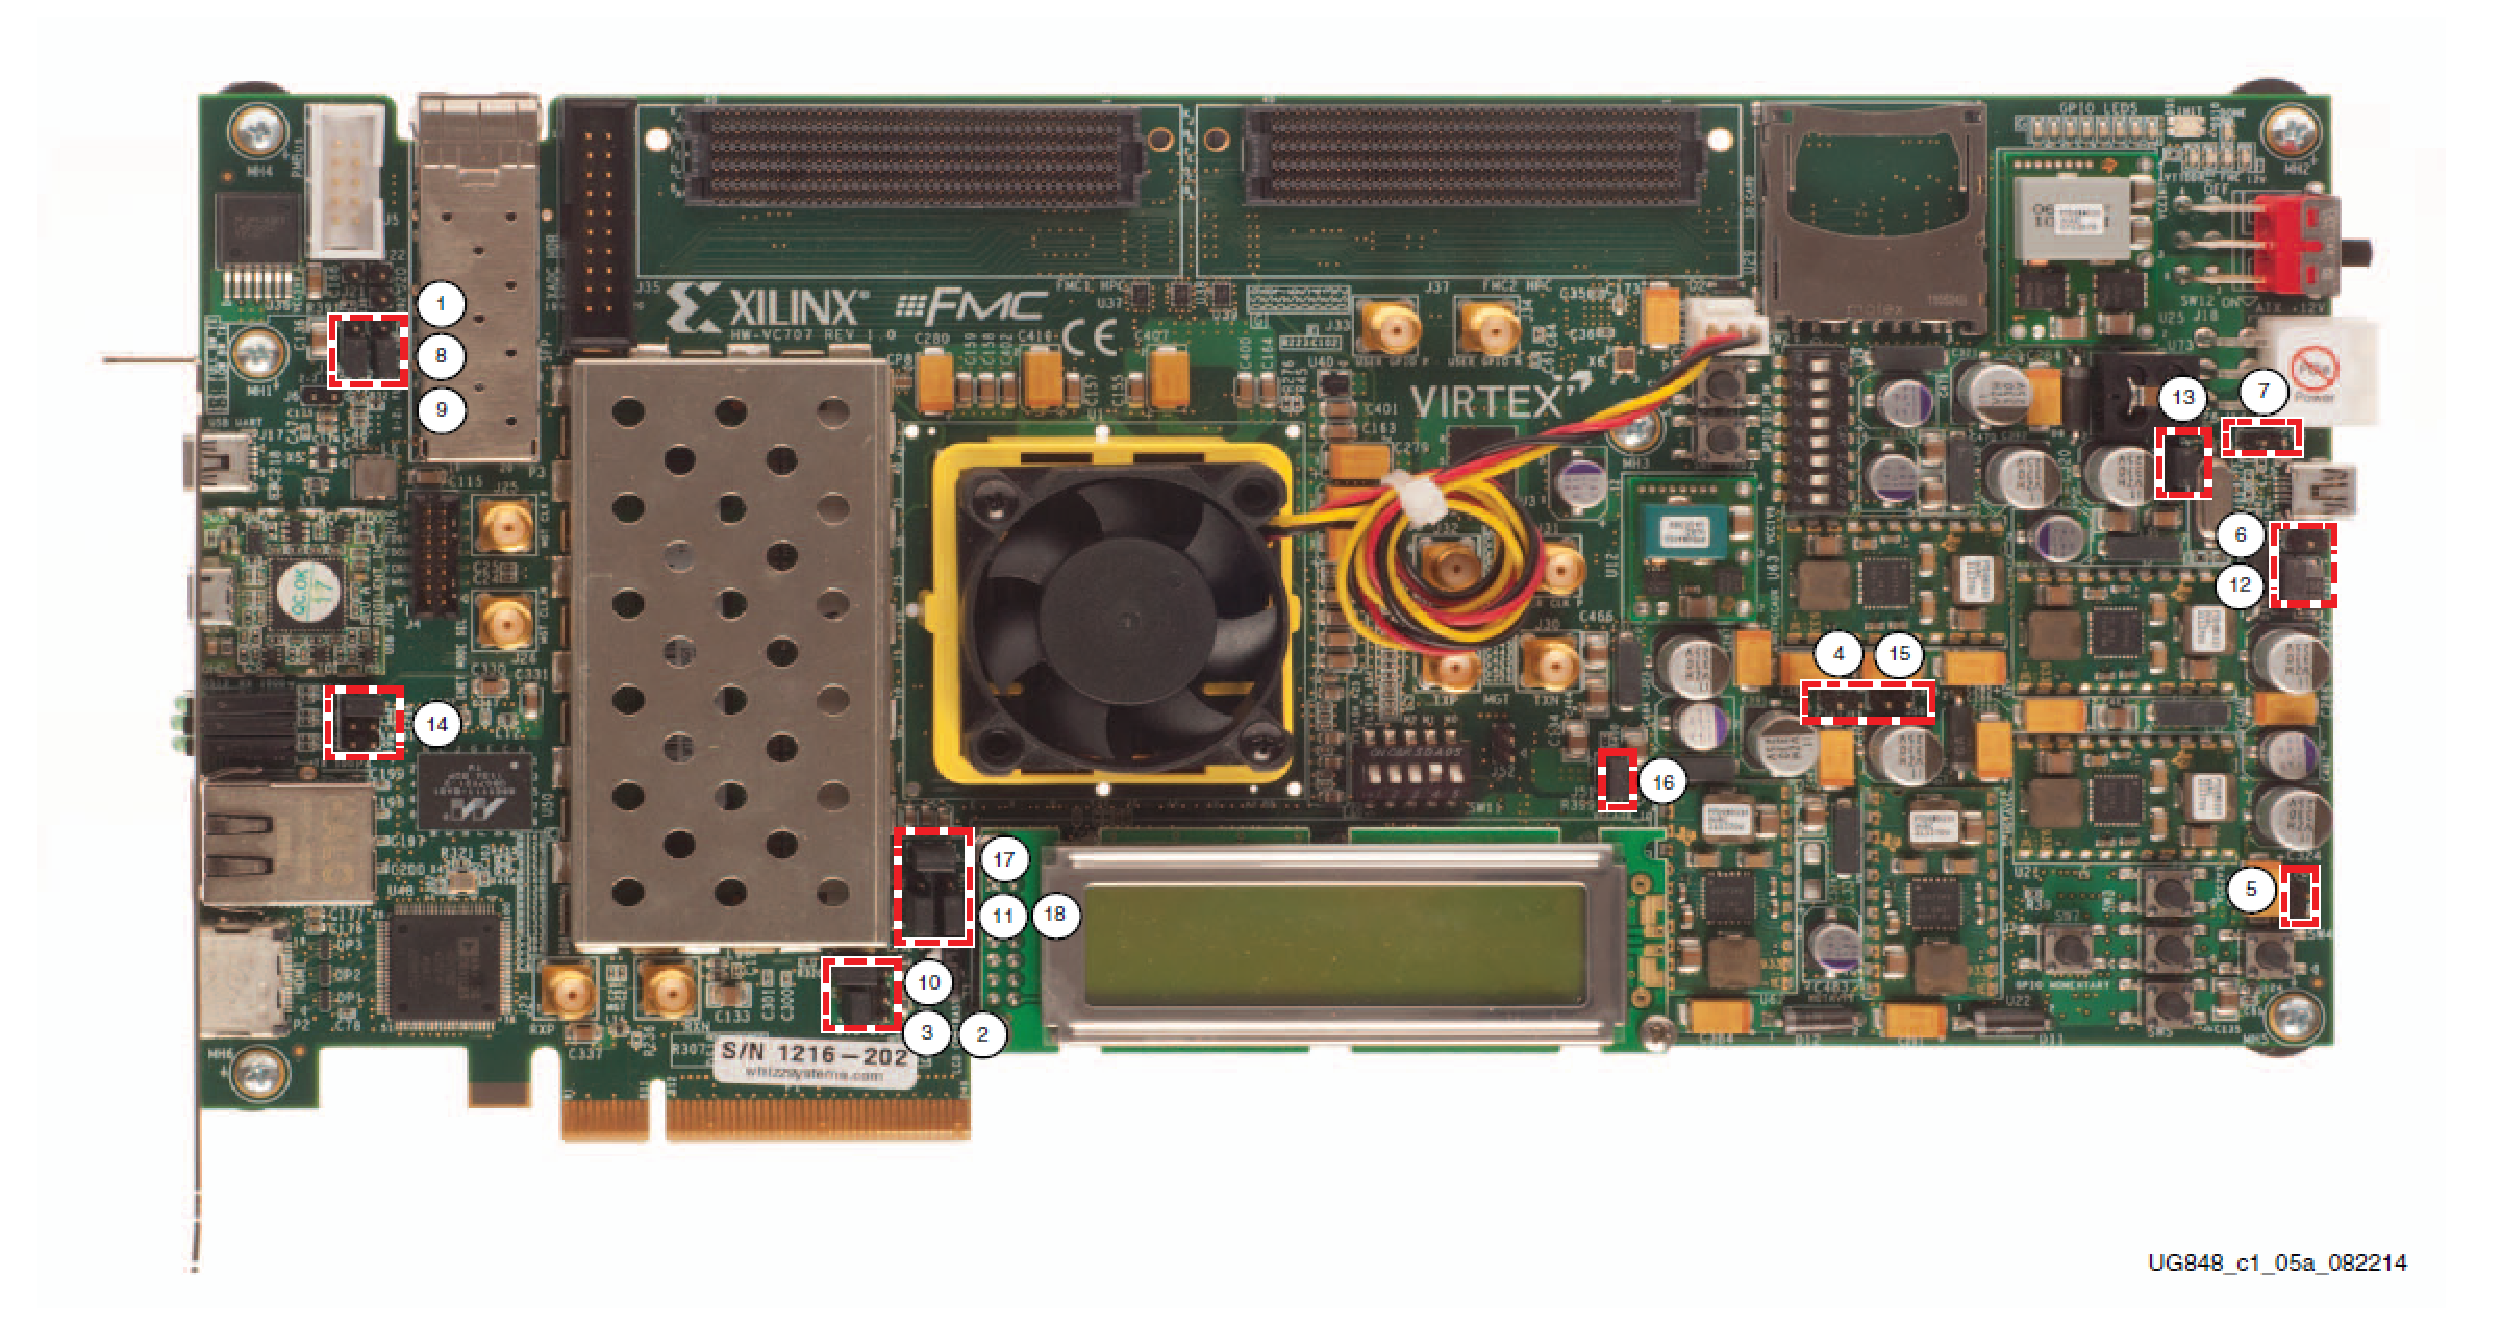
\includegraphics[width=0.8\textwidth]{./figures/vc707}
    \caption{ VC707 development board from \cite{xilinx:vc707}.
    \label{fig:vc707}}
\end{figure}

\subsection{IP Cores}

Xilinx Design Tools have a methodology of development which uses IP blocks,
called UltraFast Design Methodology \cite{xilinx:ultrafast}. In this workflow,
it is possible to develop some functionality or block and sell the right to use
it for other developers, fact which makes development a lot faster and easier.

Xilinx provide IP cores for all the development boards devices and components,
thus this part aims to briefly describe the blocks used in this work. Other
companies that develop peripherals to be integrated with Xilinx FPGAs also have
to develop and provide their own IP cores, like the FMCOMMS22 board which has its
own IP.

In Figure \ref{fig:setupip} the IP interconnections in this work, in the blue
part there are the IPs instantiated in the FPGA fabric, their role in the setup
will be explained in the following paragraphs. The core of the peripheral
control is a processor that was instantiated in the FPGA, the Microblaze. The
Microblaze role in the system developed in this work is basically to initialize
all the software drivers, configure such drivers and execute interrupt
routines. The peripherals are connected to the microblaze processor by the AXI
interconnect \cite{xilinx:axiconn}.

%figura do setup com diagrama de blocos
\begin{figure}[htbp]
    \centering
    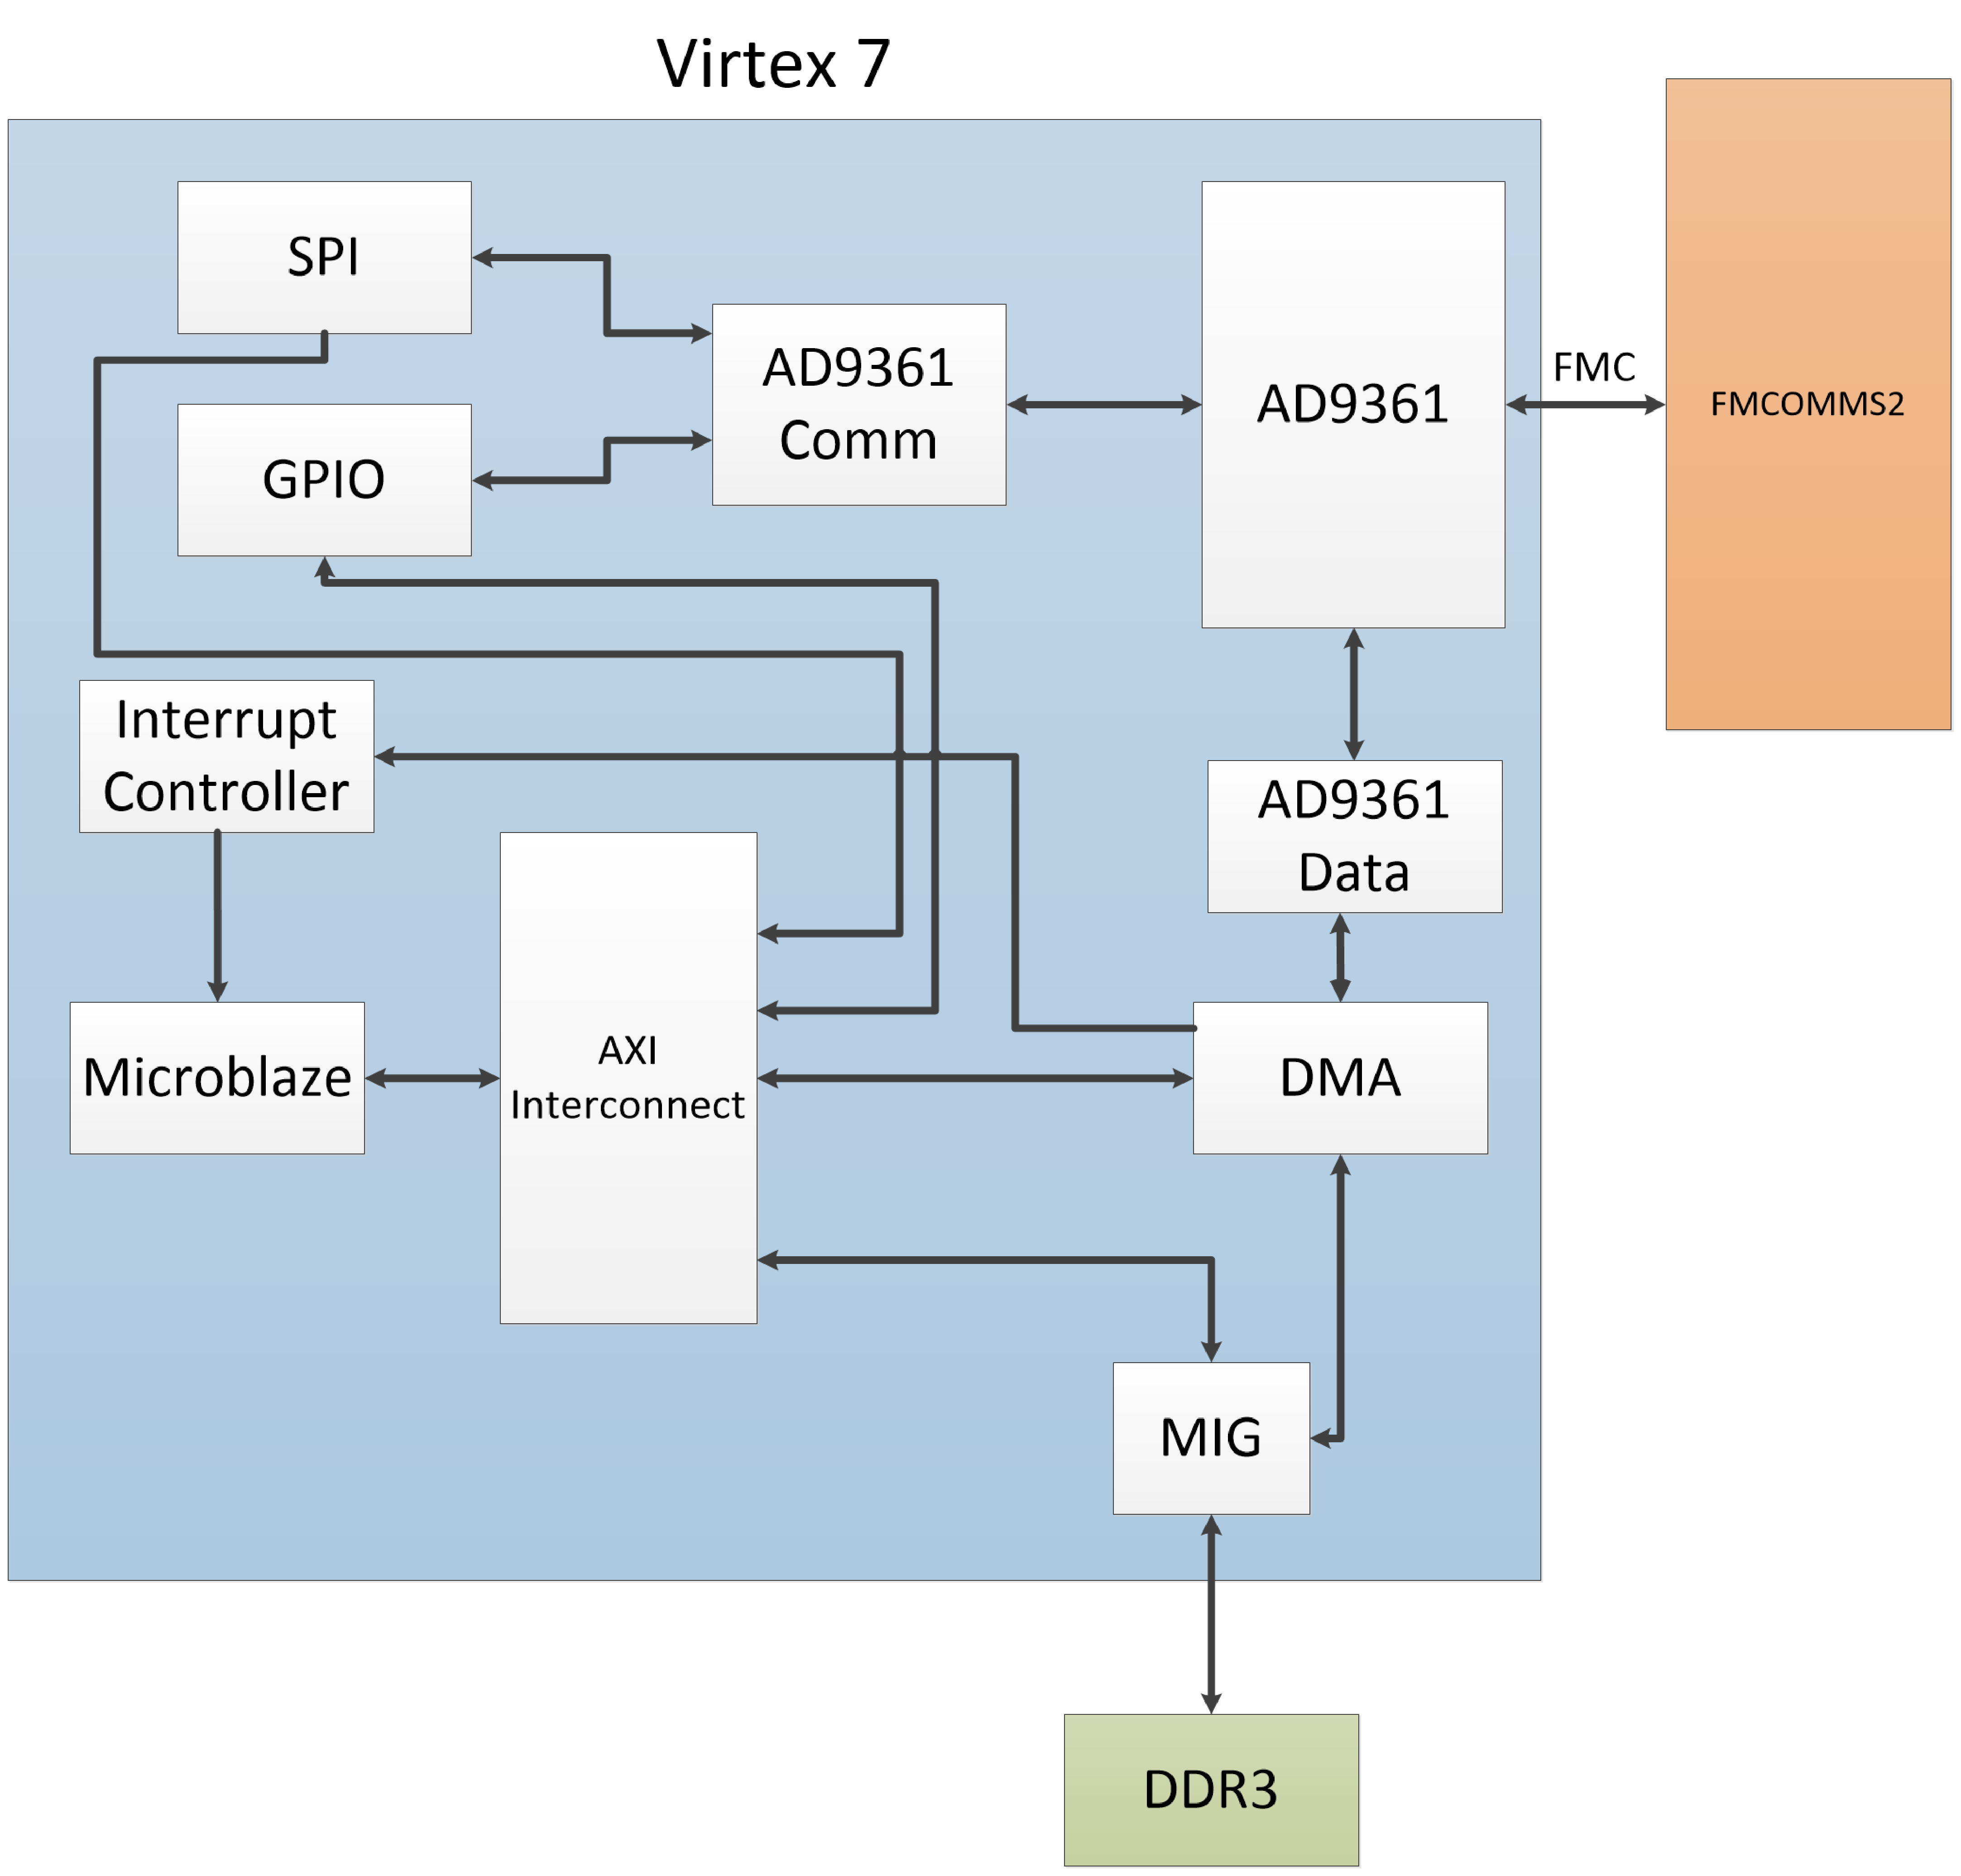
\includegraphics[width=0.75\textwidth]{./figures/setup_ip}
    \caption{ Setup components block diagram.
    \label{fig:setupip}}
\end{figure}


The DMA is the core which makes possible reading and writing from the memory in
a very fast rate \cite{xilinx:axidma}. There are various modes of operation, but
in this project the scatter gather mode is used. In this mode the reading and
writing is possible in a non-continuous memory addresses by the use of block
descriptors which stores the begin address of the reading or writing  from/into
memory, the size of the data to be read or write from/into the memory and the
address for the next block and then, DMA goes through all initialized blocks,
reading or writing.

The MIG (memory interface generator) creates a software and hardware interface
to the DDR3 memory inside the FPGA board \cite{xilinx:mig7}. Since the DDR3
module is a common SODIMM DDR3 card, there is the need to use such interface, as
can be seen in Figure \ref{fig:vc707}. In this work the MIG is also use to
generate some reference clocks for other peripherals like Microblaze and AD9361
IP core.

The SPI is a communication protocol and this core implements this protocol
inside the FPGA fabric, \cite{xilinx:axiquadspi}. In this work the SPI core
is used to write/read registers in the \emph{FMCOMMS2} board. It is
initialized and controlled by software.

GPIO stands for General Purpose Input and Output, this core implements general
purpose pins which can be configured via software to act as an input or output
pin, or even both according to \cite{xilinx:axigpio}. For this project
specifically, the GPIO core is used to make real-time operations in the AD9361
internal state-machine and for reset.

UART is also a communication protocol and stands for universal asynchronous
receiver and transmitter. The UART IP core implements such protocol in the
FPGA for USB or serial communication, according to \cite{xilinx:axiuart}. In
this work, it is used for debugging purposes, all the standard I/O form the
software comes from the UART. It is possible to read error and status
printings sent serially by the software running in the soft processor
(Microblaze).

%--------------------------------FMCOMMS2---------------------------------------
\section{Transceiver - FMCOMMS2}
\label{impl:fmcomms2}

\subsection{AD9361}
\label{trans:ad9361}

The AD9361 is a high performance RF transceiver. Its programmability and
adaptability makes it ideal for a wide range of transceiver applications
\cite{web:ad9361wiki}. This device combines an RF front end with a flexible and
configurable mixed-signal baseband section and frequency synthesizers. It
operates from 70 MHz to 6.0GHz range with supported channel bandwidths from 200
KHz to 56 MHz and has two pairs of transmit and receive antennas ports (a total
of 4 ports). Figure \ref{fig:ad9361func} shows a functional block diagram of the
AD9361 chip, in this figure it is possible to observe the logic and physical
interfaces highlighting the basic components of both, such as the transmitting
and receiving interfaces (in red), which represent the physical connections with
antennas or cables. The Transmitting and receiving oscillators and converters
are also present, DAC and ADC respectively (in blue), which make the process of
transform information to a waveform and vice versa. The logic data interface is
also present in this figure along with the control and communication interface,
with SPI and GPIO (in green).The circuit can also be fed by an external clock
reference from differential port XTALp/XTALn.

\begin{figure}[htbp]
    \centering
    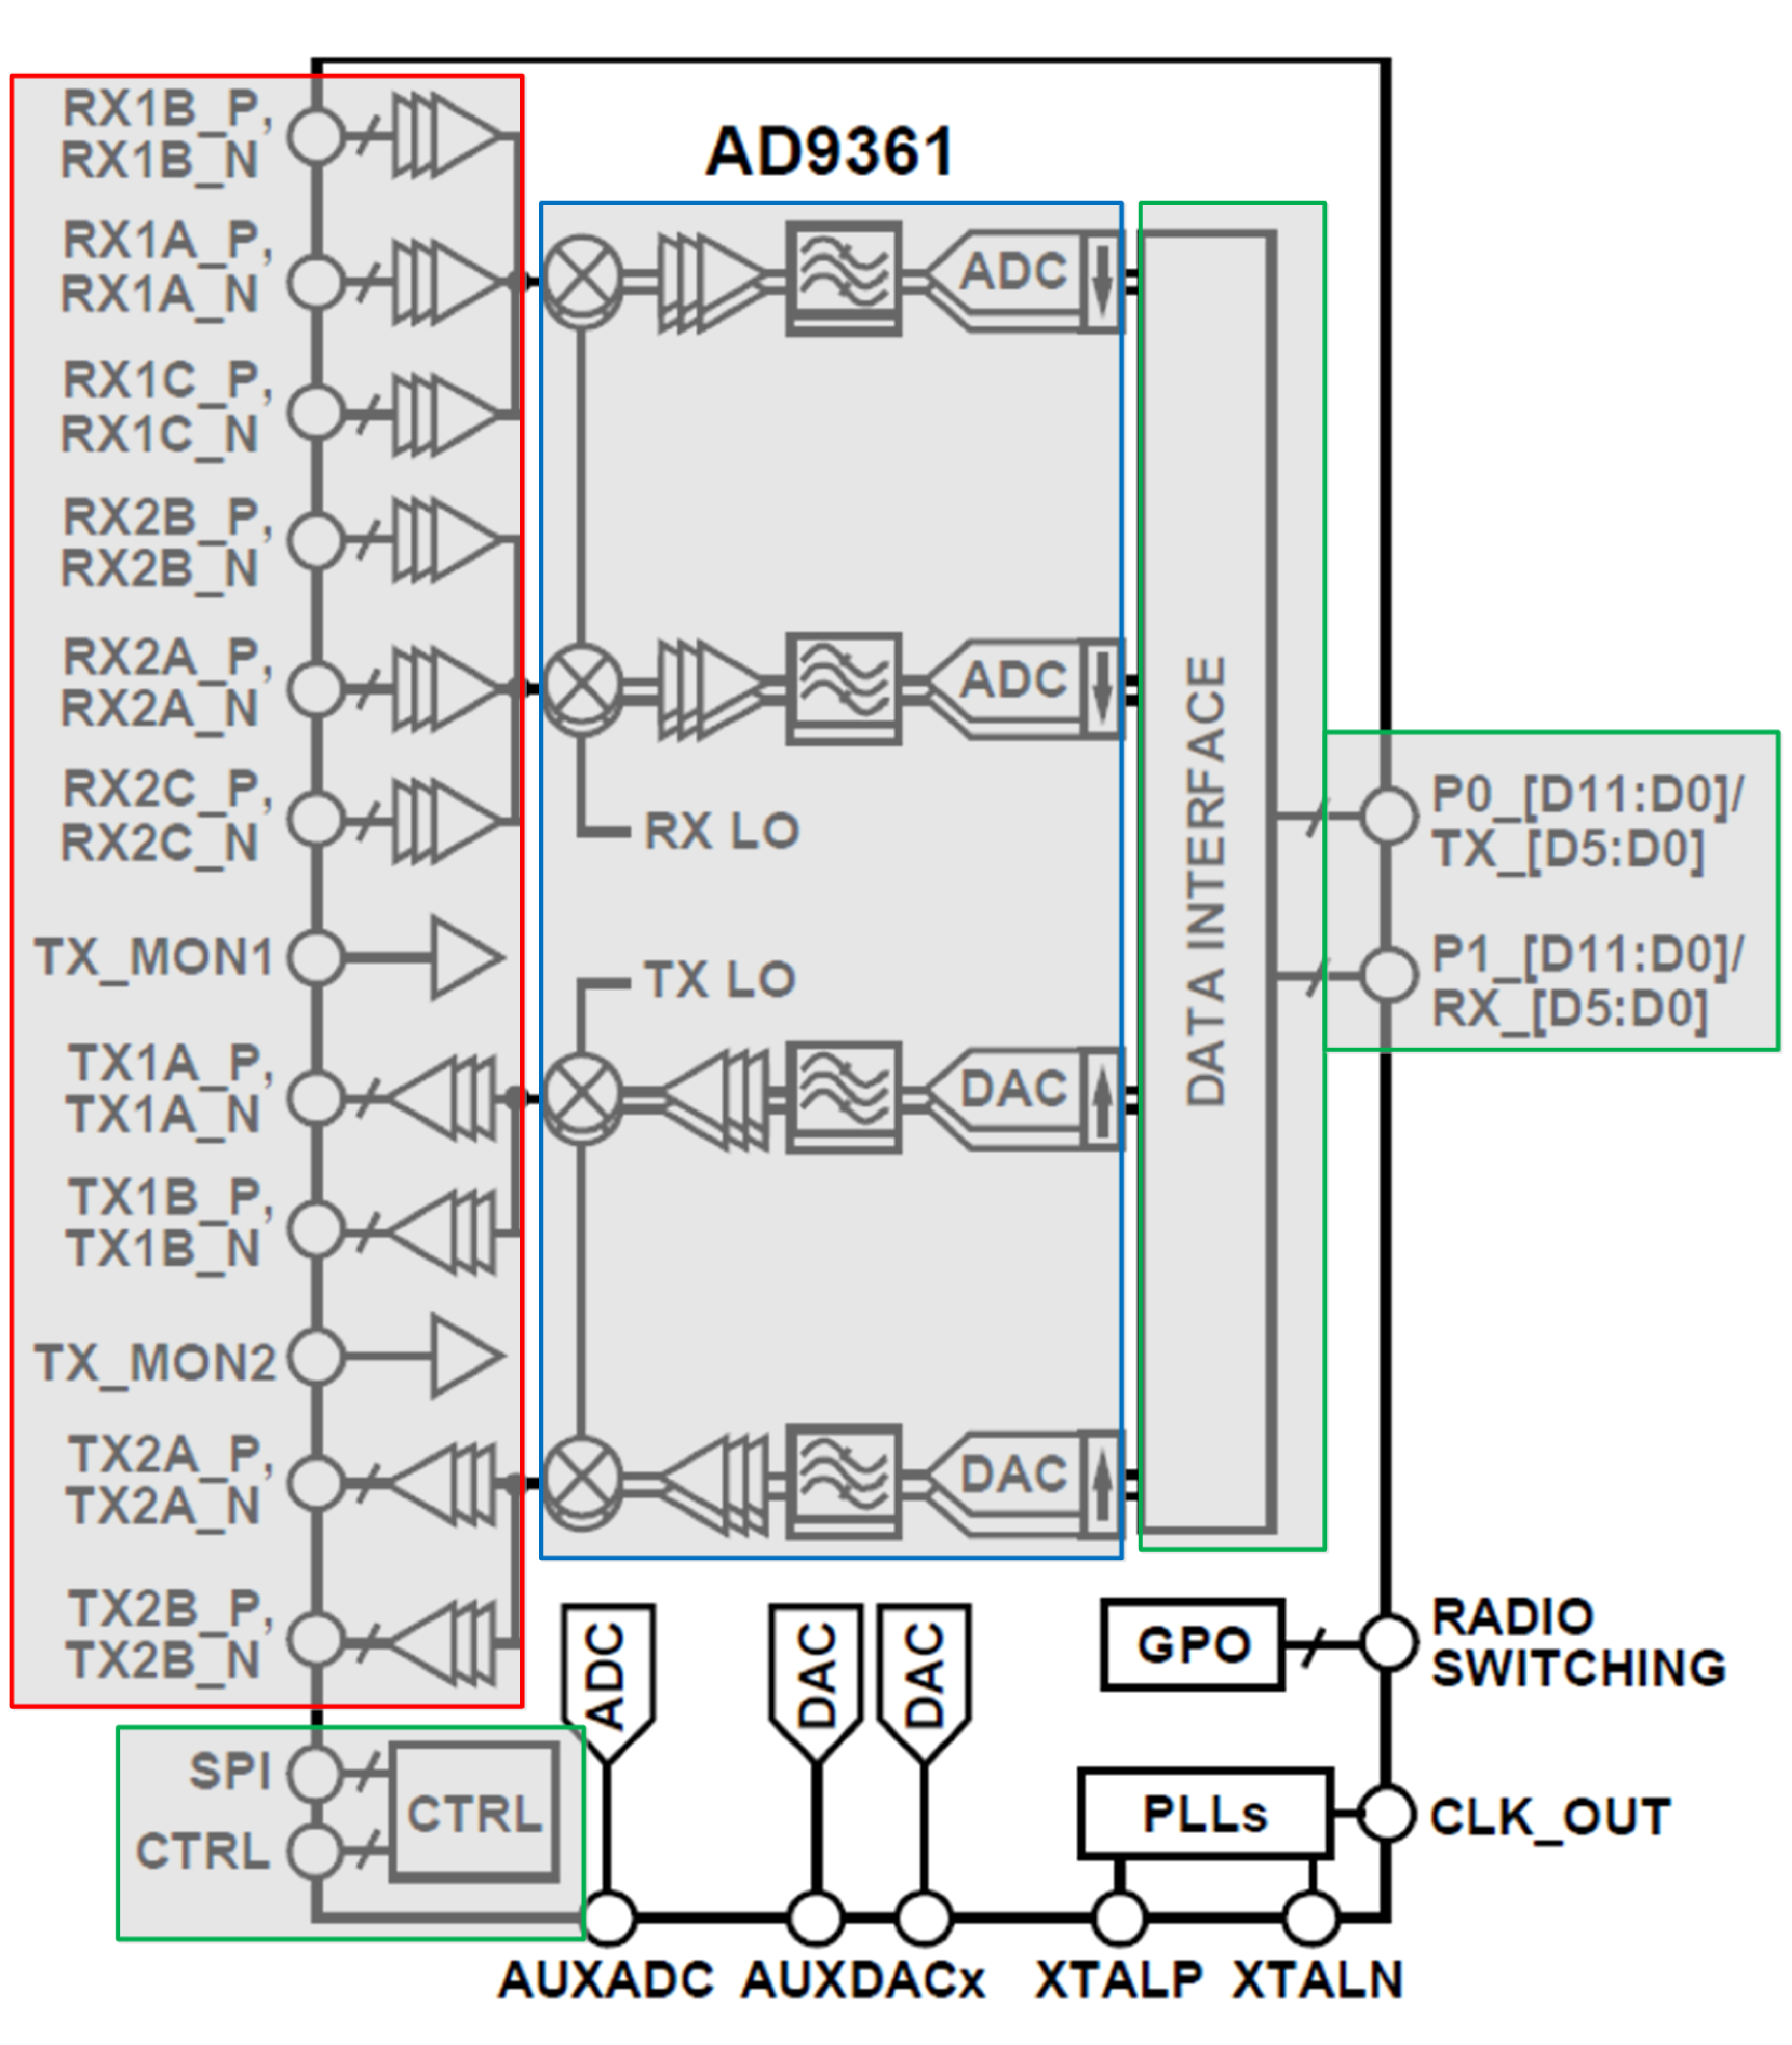
\includegraphics[width=0.55\textwidth]{./figures/ad9361_funcbd}
    \caption{ AD9361 functional block diagram.
    \label{fig:ad9361func}}
\end{figure}

\subsubsection{Receiver}

The receiver section has all the blocks necessary to receive analog RF signals
and convert them to digital data which can be used by the Baseband Processor
(BBP), as can be ssen in Figure \ref{fig:rxchain}. There are two independently
controlled channels that share same frequency synthesizer. This characteristic
allows the AD9361 to operate in  2x2 MIMO systems.

Each channel has 3 inputs that can be multiplexed into the signal chain, making
possible to use the AD9361 into systems with multiple antenna inputs. The
Receiver is a direct conversion system that contains a low noise amplifier
(LNA), followed by a matched in-phase and quadrature amplifier, mixers, and band
shaping filters that down converts received signals to baseband for
digitization. The
receiver signal passes down-converted complex baseband signals composed by
in-phase and quadrature terms (I and Q) to the baseband (BB) processing unit in
the receiver. The BB section is composed by two programmable low-pass filters
(TIA LPF and BB LPF), 12-bit ADC and four stages of decimating filters (HB3,
HB2, HB1/DEC1 and PROG RX FIR in Figure \ref{fig:rxchain}).

The gain control is achieved by a preprogrammed gain index map, a lookup table
for example. This map distributes the gain in order to achieve optimal
performance at each level. This optimal behavior can be achieved by enabling
automatic gain factors to produce the needed data rate.

\begin{figure}[htbp]
    \centering
    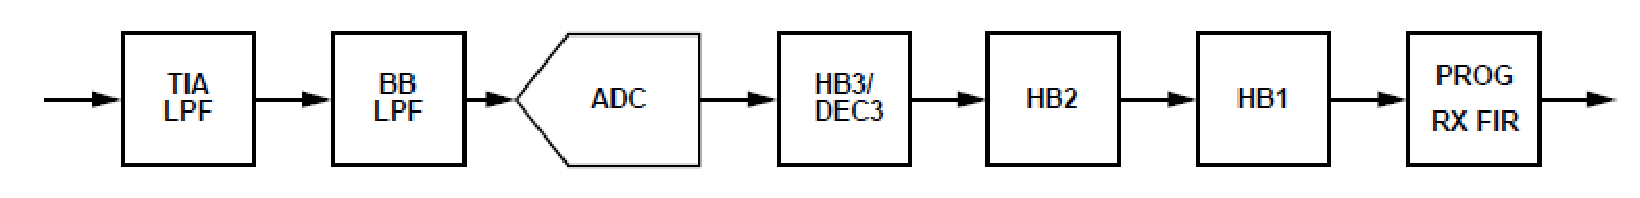
\includegraphics[width=0.85\textwidth]{./figures/rx_chain}
    \caption{ Receiver signal path.
    \label{fig:rxchain}}
\end{figure}


\subsubsection{Transmitter}

Like the receiver, the transmitter section, illustrated in Figure
\ref{fig:txchain}, contains two identical and independently controlled channels,
which share the same frequency synthesizer and provide all digital signal
processing, mixed signal and RF blocks necessary to implement a direct
conversion system from digital data to RF. The transmitter signal path receives
from the BBP 12-bit I-Q format data in the digital interface and each channel
goes through a series of additional interpolation filters that manipulates the
signal with additional filtering and data rate interpolation (PROG TX FIR, HB1,
HB2 and HB3/INT3 ) before reaching the 12-bit DAC. After all these filtering and
analog conversion steps, the I and Q signals are recombined and modulated in the
carrier frequency, which can be adjusted by changing the synthesizer frequency
\cite{ad:ad9361}.

Identical to the receiver chain, the transmitter chain has also built-in
self-calibration circuitry into each transmitting channel providing an automatic
real-time adjustment of the gain.

\begin{figure}[htbp]
    \centering
    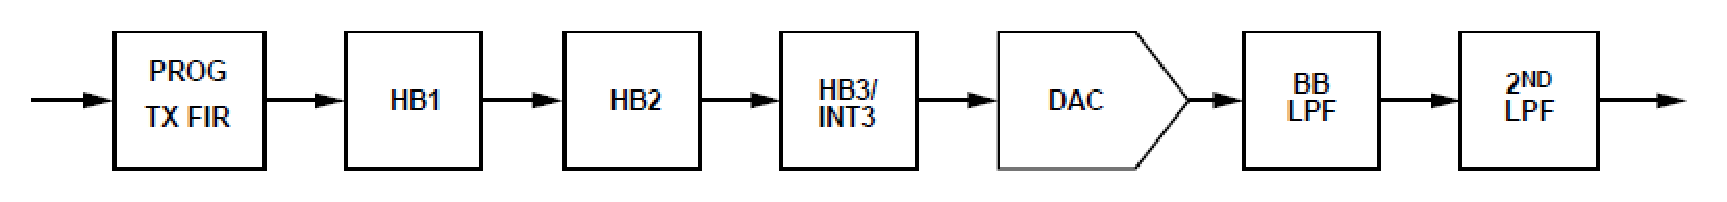
\includegraphics[width=0.85\textwidth]{./figures/tx_chain}
    \caption{ Transmitter signal path.
    \label{fig:txchain}}
\end{figure}

In Figure \ref{fig:ad9361blk} there is a figure which incorporate the previous
sections blocks into one, and then it is easier to understand the whole AD9361
block. This figure shows both transmitting chain (in red) and receiver chain (in
blue), there is 2 of each chain. Another  noteworthy aspect is that the
oscillators and all the clock chain is observed in this image (in the middle).
Another interfaces which were mentioned in Figure \ref{fig:ad9361func} are
present, such as SPI and GPIO.The data path passes through the LVDS interface
to reach FPGA logic, this interface is the physical interface in which AD9361
will integrate which the FPGA by the FMCOMMS2 FMC connector.

\begin{figure}[htbp]
    \centering
    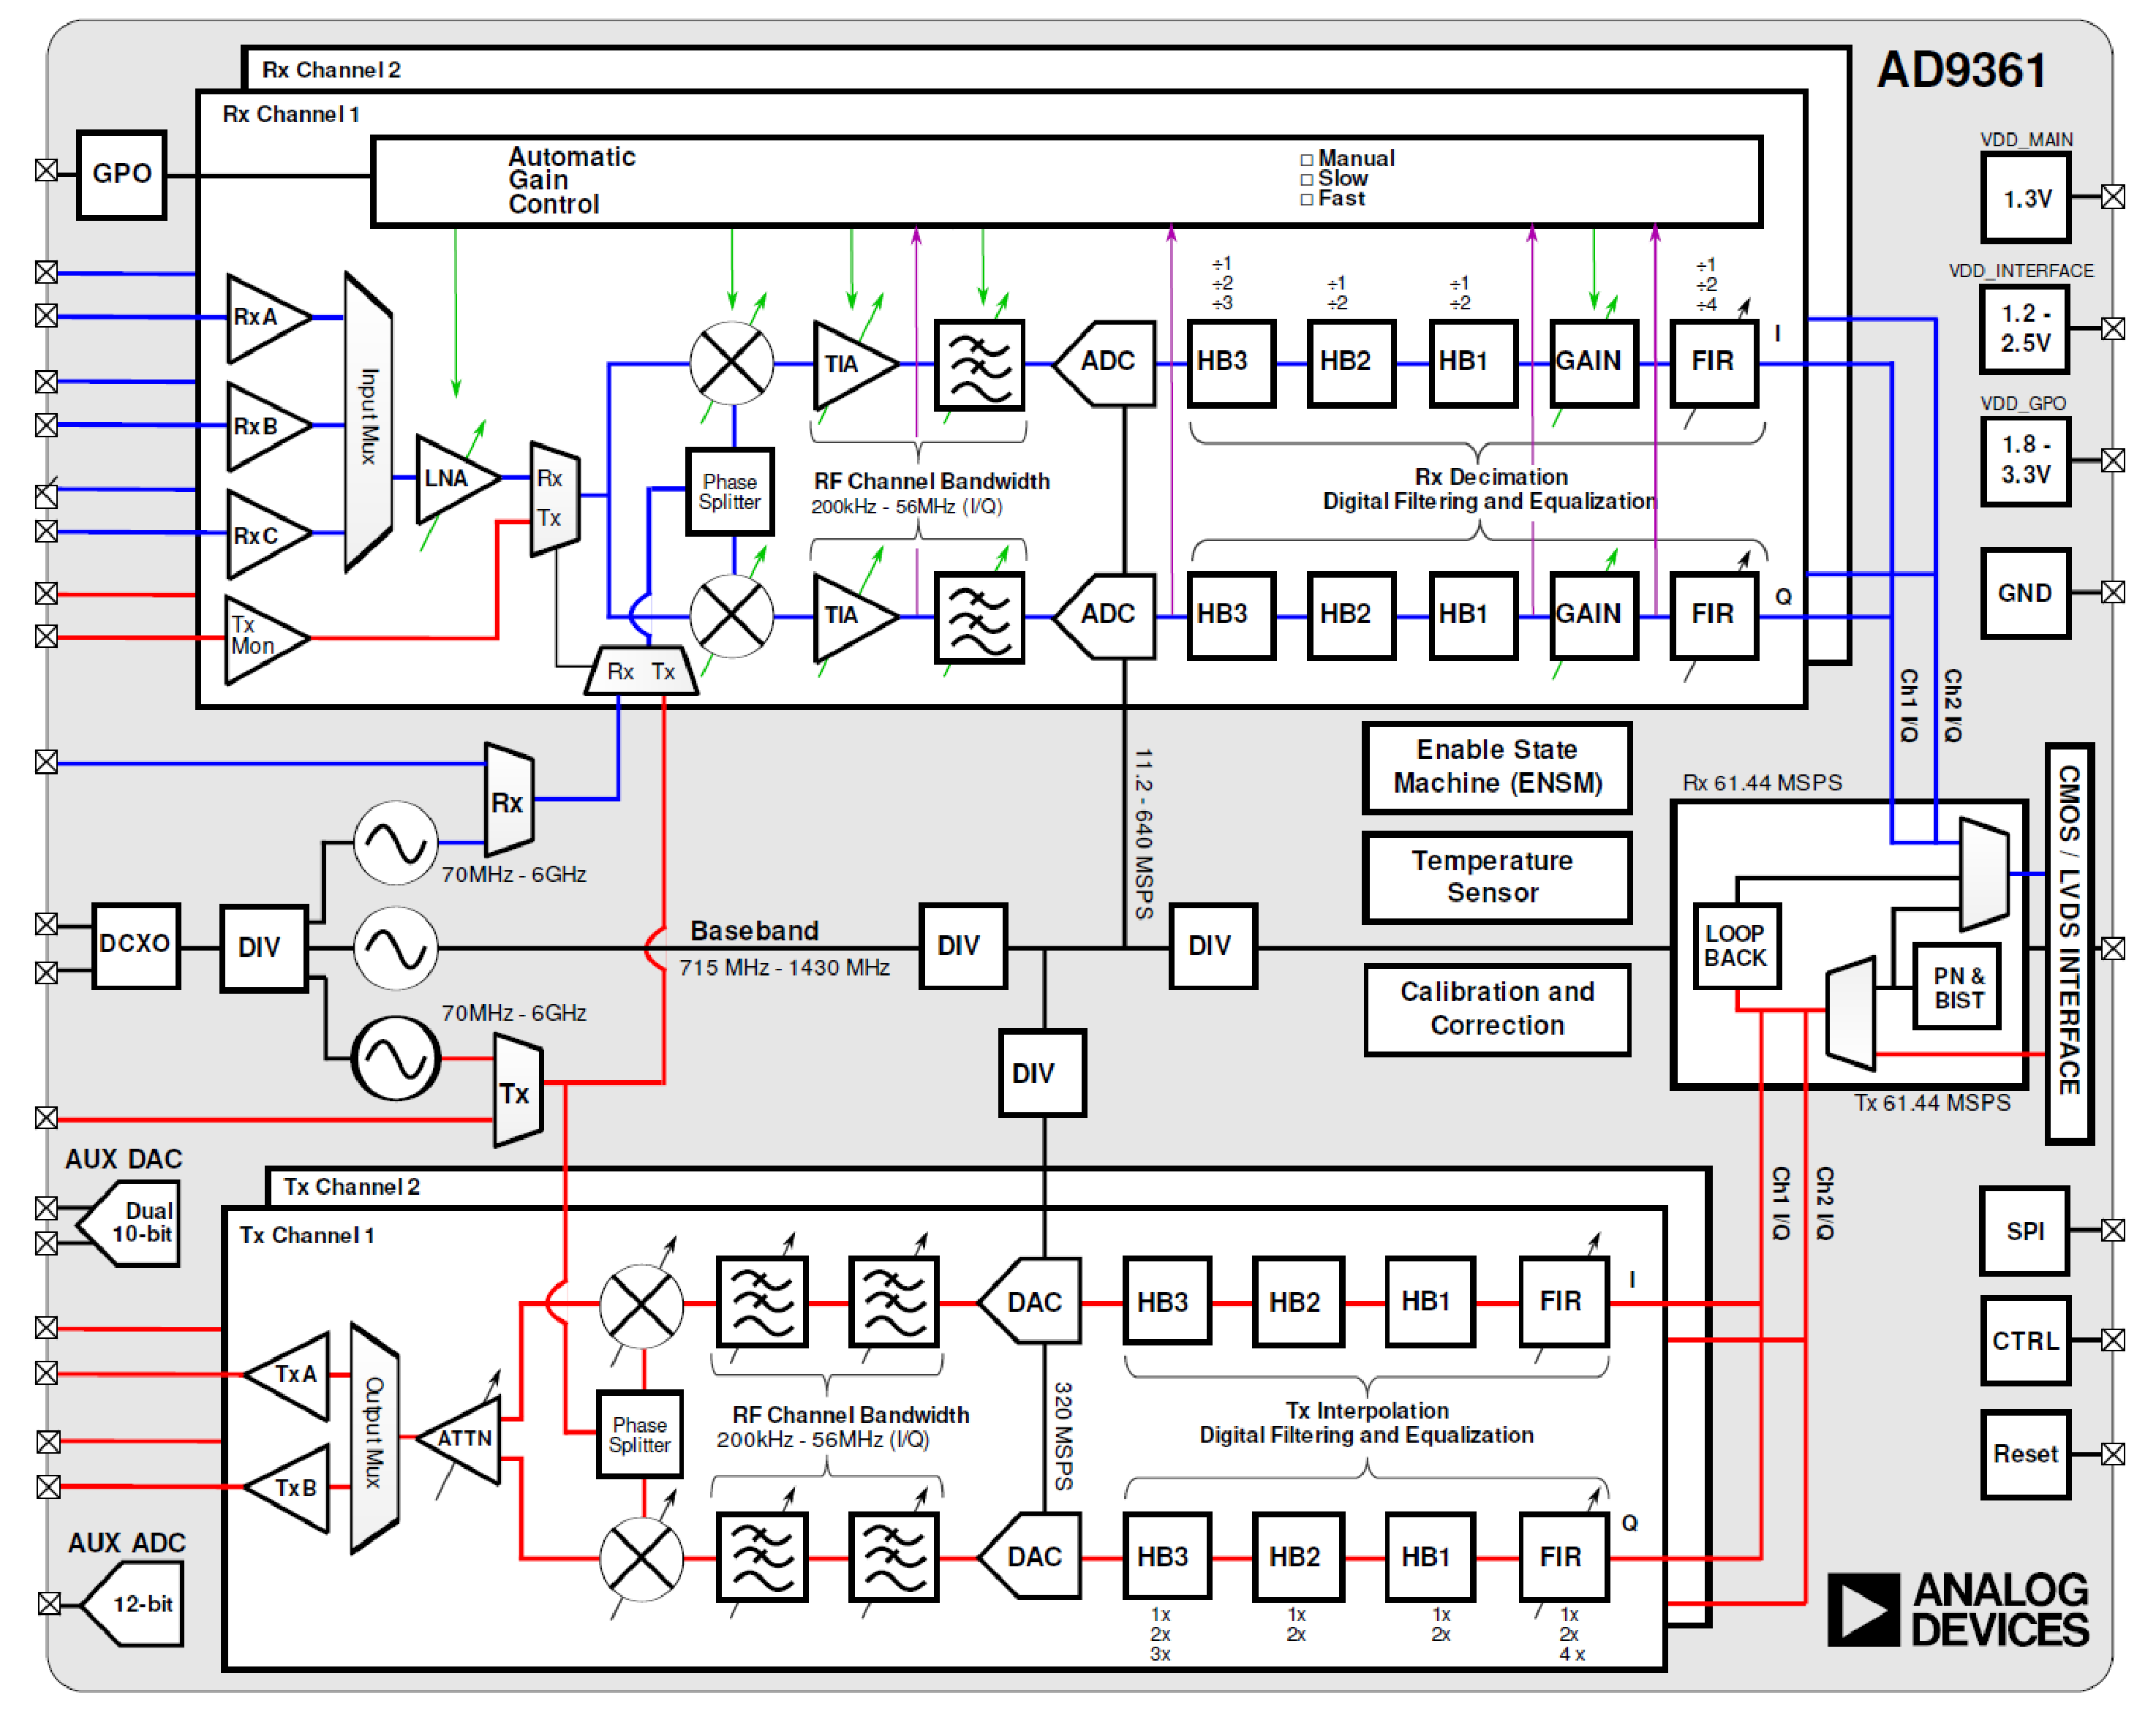
\includegraphics[width=0.95\textwidth]{./figures/ad9361_block_diagram}
    \caption{ AD9361 block diagram.
    \label{fig:ad9361blk}}
\end{figure}

\subsubsection{Filtering}

In both receiver and transmitter there are low pass filters and
decimation/interpolation filters. In the receiver the low pass filter acts in
band shaping to reduce adjacent-channel interference and the digital
interpolation/decimation filters to up/down convert from the digital baseband
rate (64.11 MSPS max) to the actual ADC (640 MSPS) or DAC (320 MSPS) rates
\cite{web:ad9361wiki}.

In both digital and analog implementations these filters impact the magnitude
and the phase in passband. This impairment must be compensated in the system,
and this compensation is usually done inside the 128-tap FIR filter. The FIR
filter is not only used for low pass filter realization but also to compensate
for magnitude and phase impacts created by the analog and digital half band
filters in the desired baseband area.

\subsubsection{Clocking}

%reescrever
The AD9361 has a series of internal phase-locked loops (PLL) to generate and
manipulate clock signals. There are $fractional-n$ PLLs that generate the
transmitter and receiver local oscillator (LO) frequencies and there are the
baseband PLL (BBPLL) used for the data converters, digital filters and I/O
ports. All the frequency signals are generated using these PLL clock outputs.

All the PLL requires is a reference clock input and for this there is the
digitally controlled oscillator (DCXO), which crystal is controlled by an
on-chip programmable capacitor \cite{web:ad9361wiki}. This capacitor can tune
the crystal frequency variance out of the system, resulting in a more accurate
reference clock from which all other frequency signals are generated. Having a
precision of +/- 6 ppm it results in a more accurate reference clock and can be
used, if needed, for synchronization purposes. The behavior of the DCXO
function can be seen in Figure \ref{fig:dcxo}, which shows one curve for each
valor of coarse adjust, this image crafted by empirically collecting of values
\cite{ad:ad9361}. This function can also be used together with the on-chip
temperature sensor to provide temperature compensation depending environment in
which the chip will be used \cite{ad:ad9361}.

For the reference clock there are two options, one is a dedicated crystal
oscillator (from 19 to 50 MHz), which is embedded in the FMCOMMS2 development
board that will be described in the next section. Other option is the use of an
external clock reference. In this option the BTS can operate in the clock (from
10 MHz to 80 MHz) before sending it to the AD9361, which is better depending in
the synchronization requirements.

\begin{figure}[htbp]
    \centering
    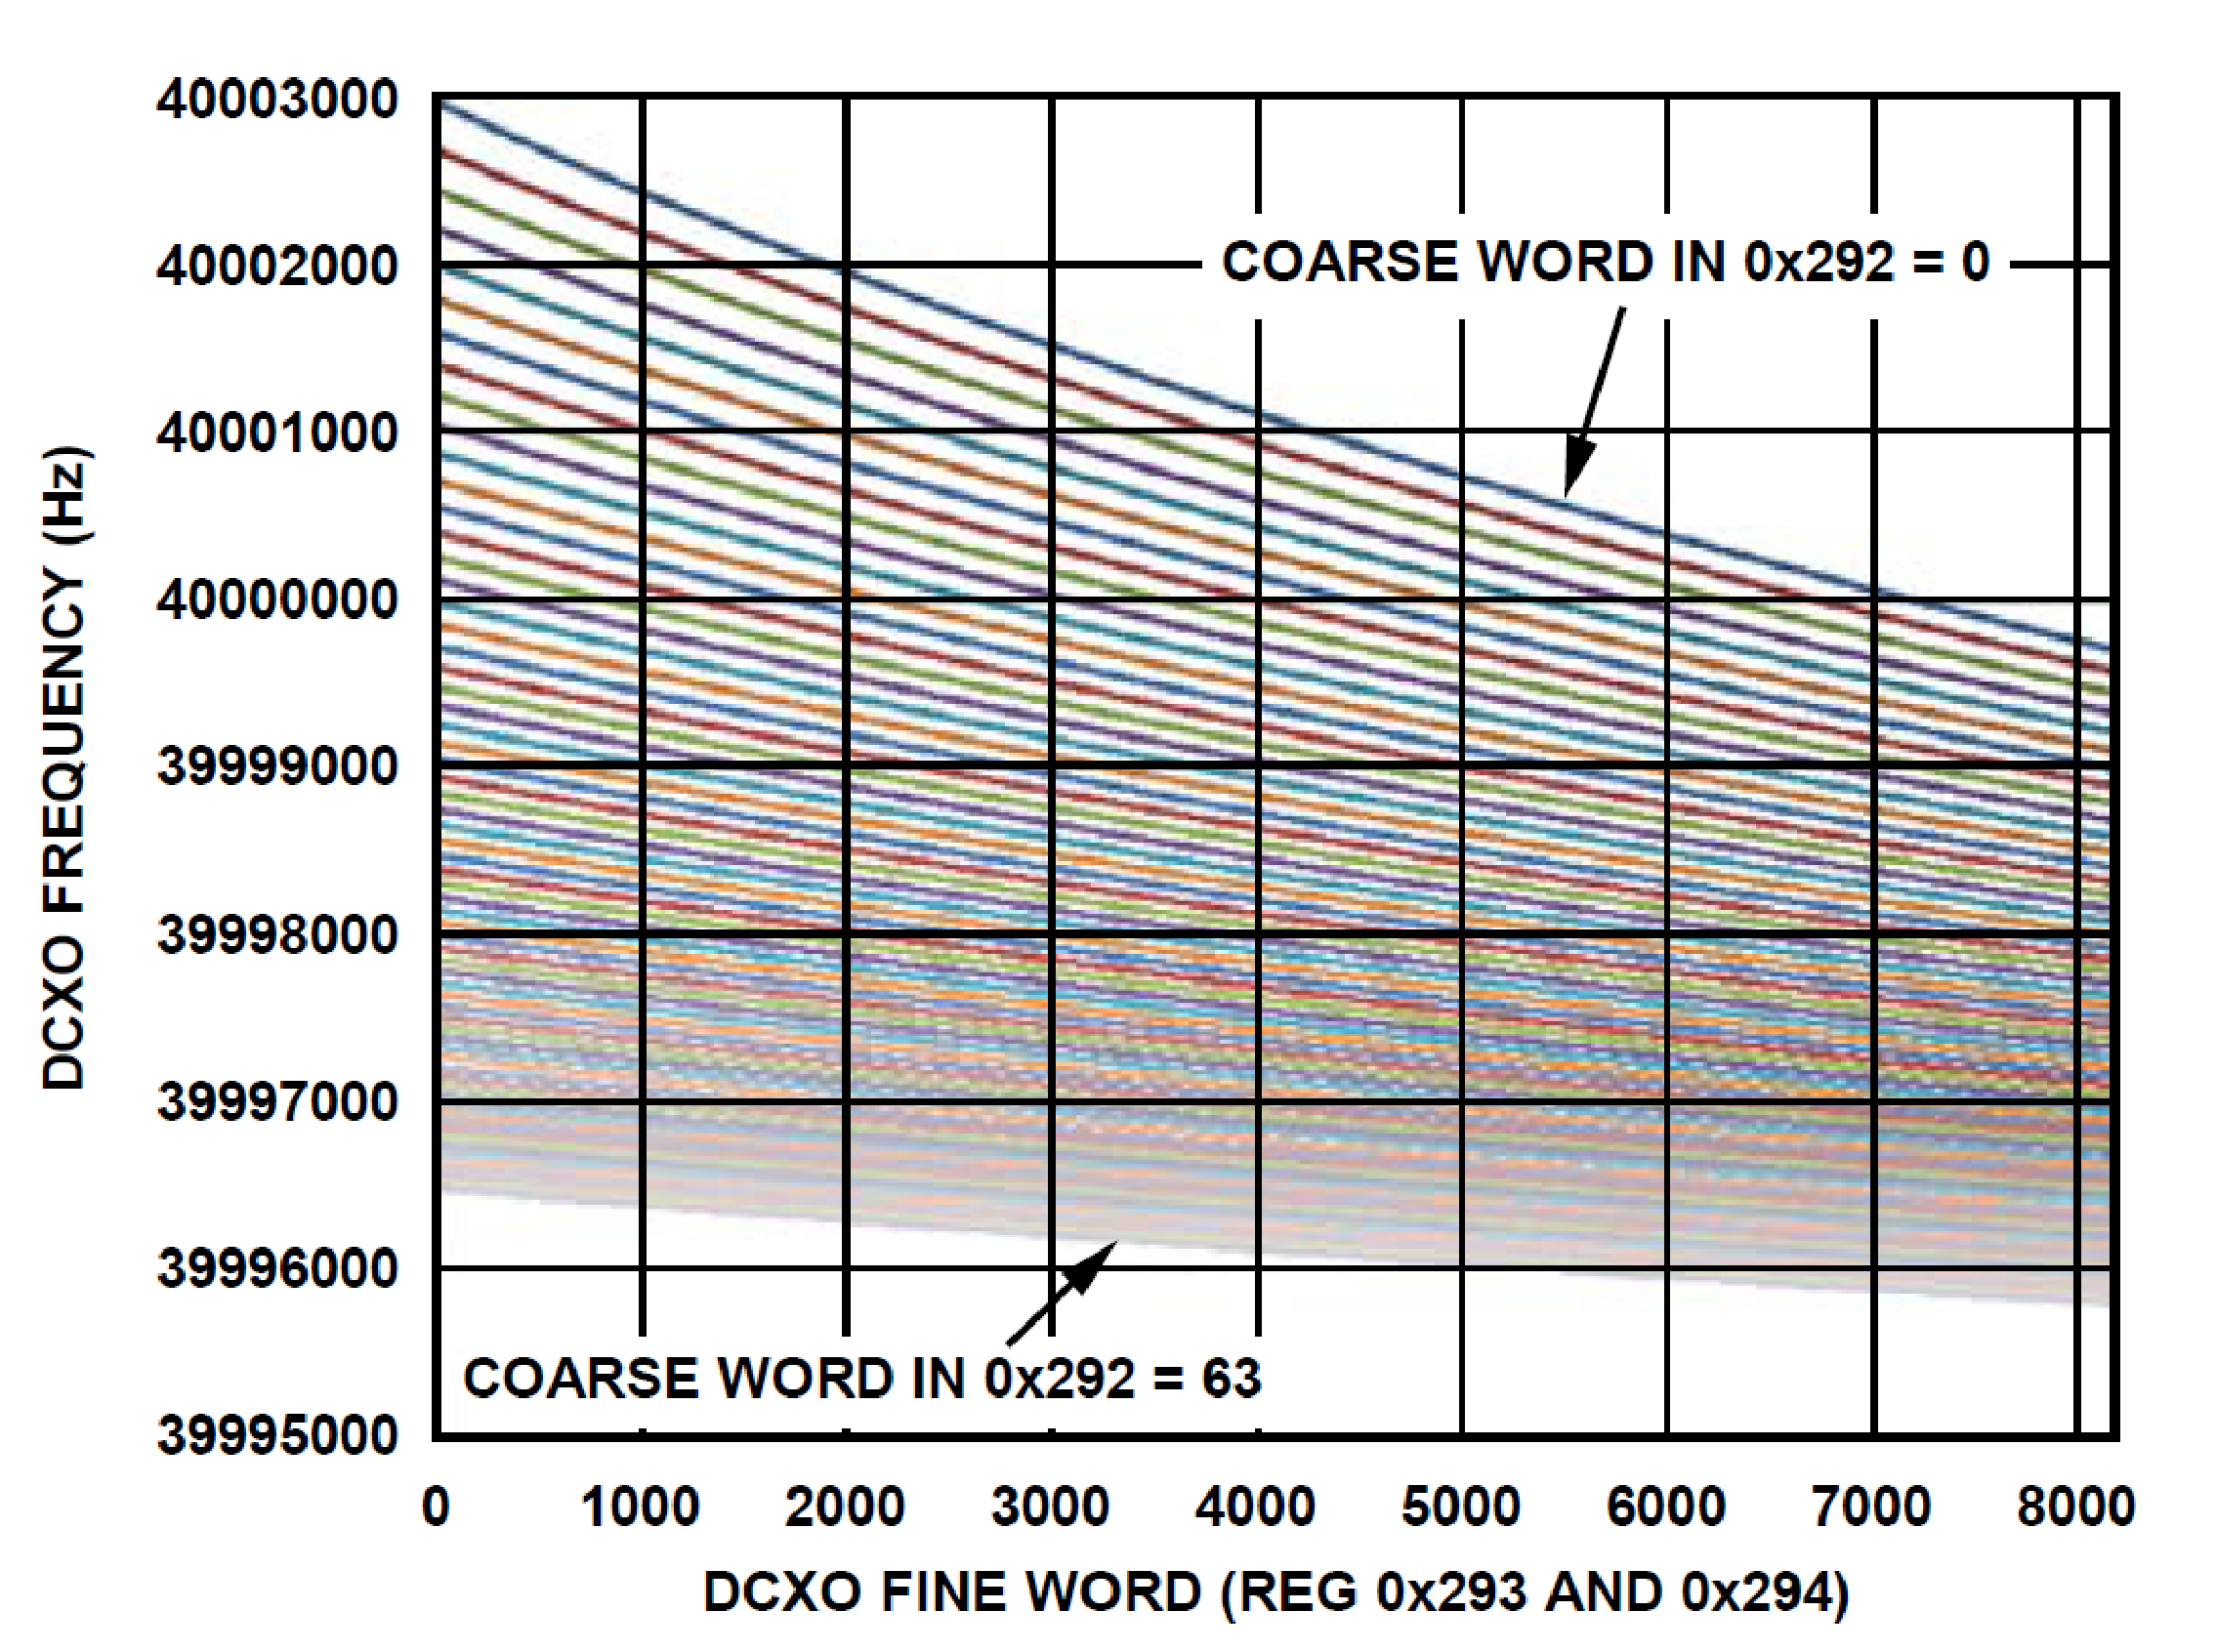
\includegraphics[width=0.55\textwidth]{./figures/dcxo_graph}
    \caption{ DCXO behavior graph.
    \label{fig:dcxo}}
\end{figure}


\subsection{FMCOMMS2}
\label{trans:fmcomms2}

FMCommS2 is basically evaluation board for the AD9361 that has a FMC connector
for interfacing with the BBP (usually FPGA). It has 5 SMA connectors, 2 for Rx,
2 for Tx and one for external reference clock input. The FMComms2 provides a 2x2
RF configuration, extended from the AD9361, as seen in Figure \ref{fig:fmcomm}.

The FMComms2 is a transceiver intended for use in RF applications such  as 3G or
4G EnodeB or SDR. Its programmability and wide-band capability make it ideal for
broad range of transceiver applications and make it very attractive for the new
C-RAN paradigm. The board and some components can be seen in Figure
\ref{fig:fmcomm}.

\begin{figure}[htbp]
    \centering
    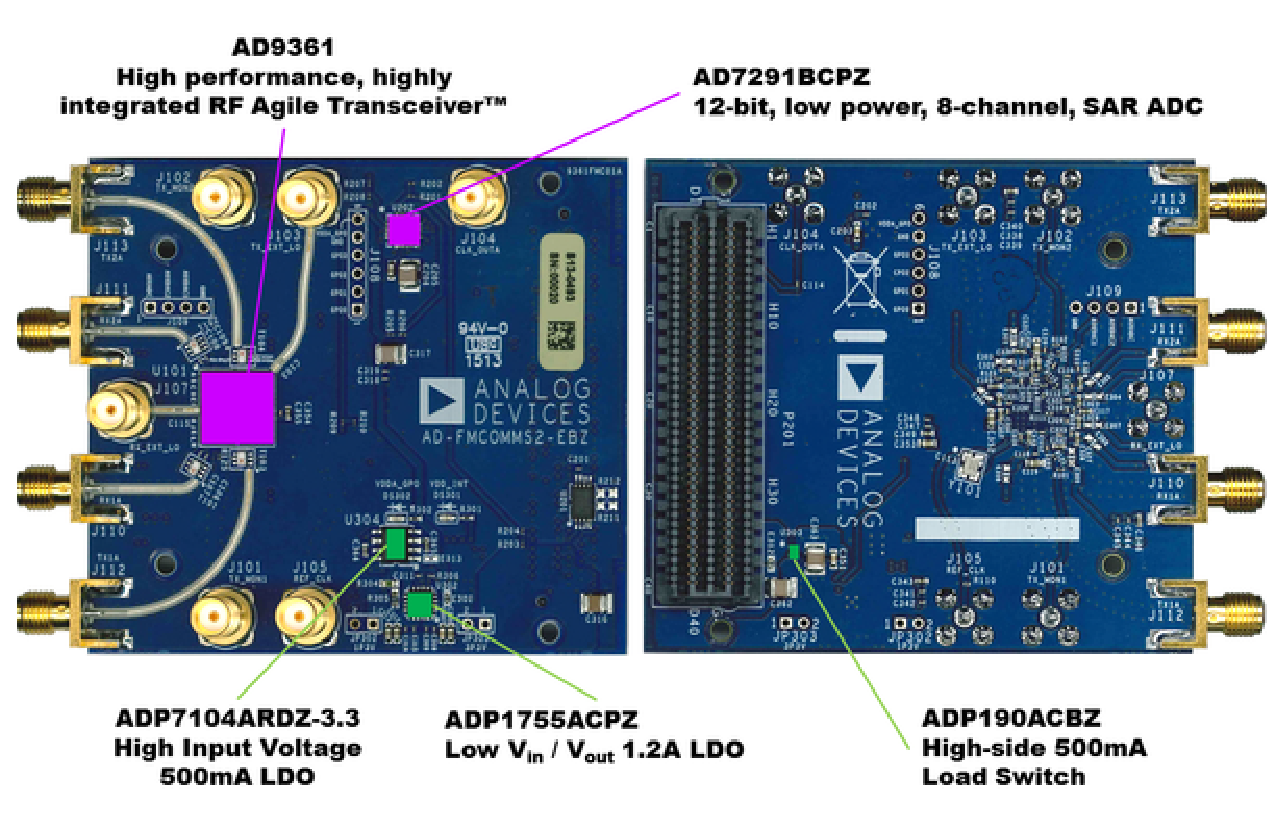
\includegraphics[width=0.75\textwidth]{./figures/fmcomms2_pic}
    \caption{ FMCOMMS2 and its components.
    \label{fig:fmcomm}}
\end{figure}

Figure \ref{fig:fmcommbd} shows the basic integration between FPGA and FMCOMMS2,
for such there is an IP developed by Analog Devices to map all the signals to
the correct physical pins in the FMC connector. This figure also shows the
basic IP infrastructure needed to control and communicate between the FPGA and
FMCOMMS2, such as Processor (Microblaze or ARM), SPI and GPIO, basically. Since
the FMCOMMS2 incorporates and extends the basic functionalities of the AD9361,
thus the data path is fully integrated into the AD9361 \cite{web:fmcomms2wiki}.

\begin{figure}[htbp]
    \centering
    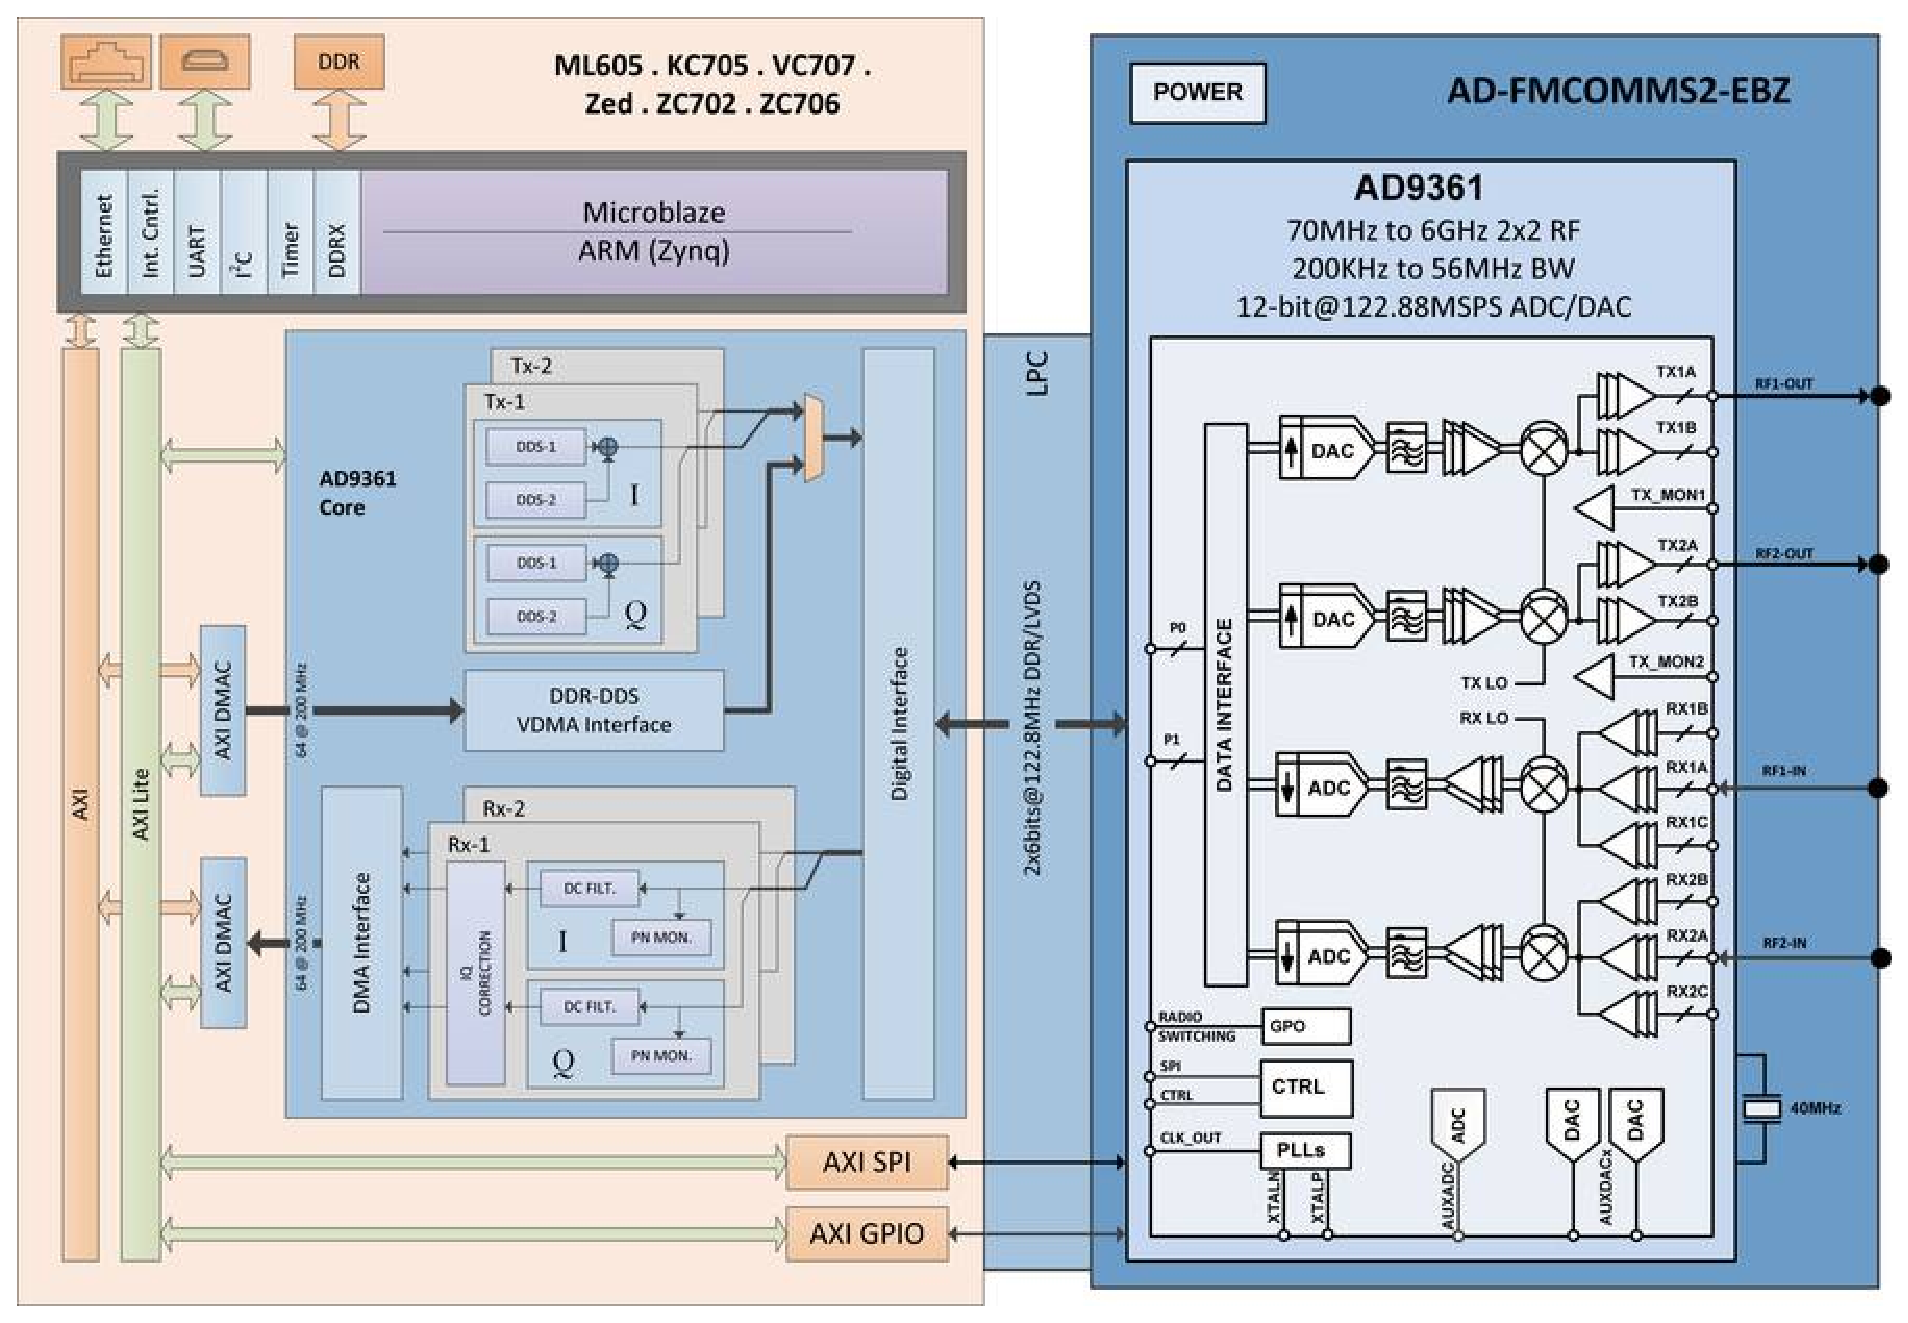
\includegraphics[width=0.95\textwidth]{./figures/fmcomms2_bd}
    \caption{ FMCOMMS2 and FPGA block diagram.
    \label{fig:fmcommbd}}
\end{figure}


\section{Setup}
\label{impl:setup}

\subsection{Overview}

To illustrate the idea of this setup and to facilitate its explanation the
transmitter and receiver chains were separated in Figure \ref{fig:txsetup} and
Figure \ref{fig:rxsetup}. These figures show a high level block diagram of the
signal flow until it becomes a waveform (transmitter) or a binary stream
(receiver). The functionalities of the  DAC-DMA interface and DAC Interface
blocks in Figure \ref{fig:txsetup} and the ADC interface block in Figure
\ref{fig:rxsetup} are explained in Subsection \ref{subs:dataif}.

%tx block diagram
\begin{figure}[htbp]
    \centering
    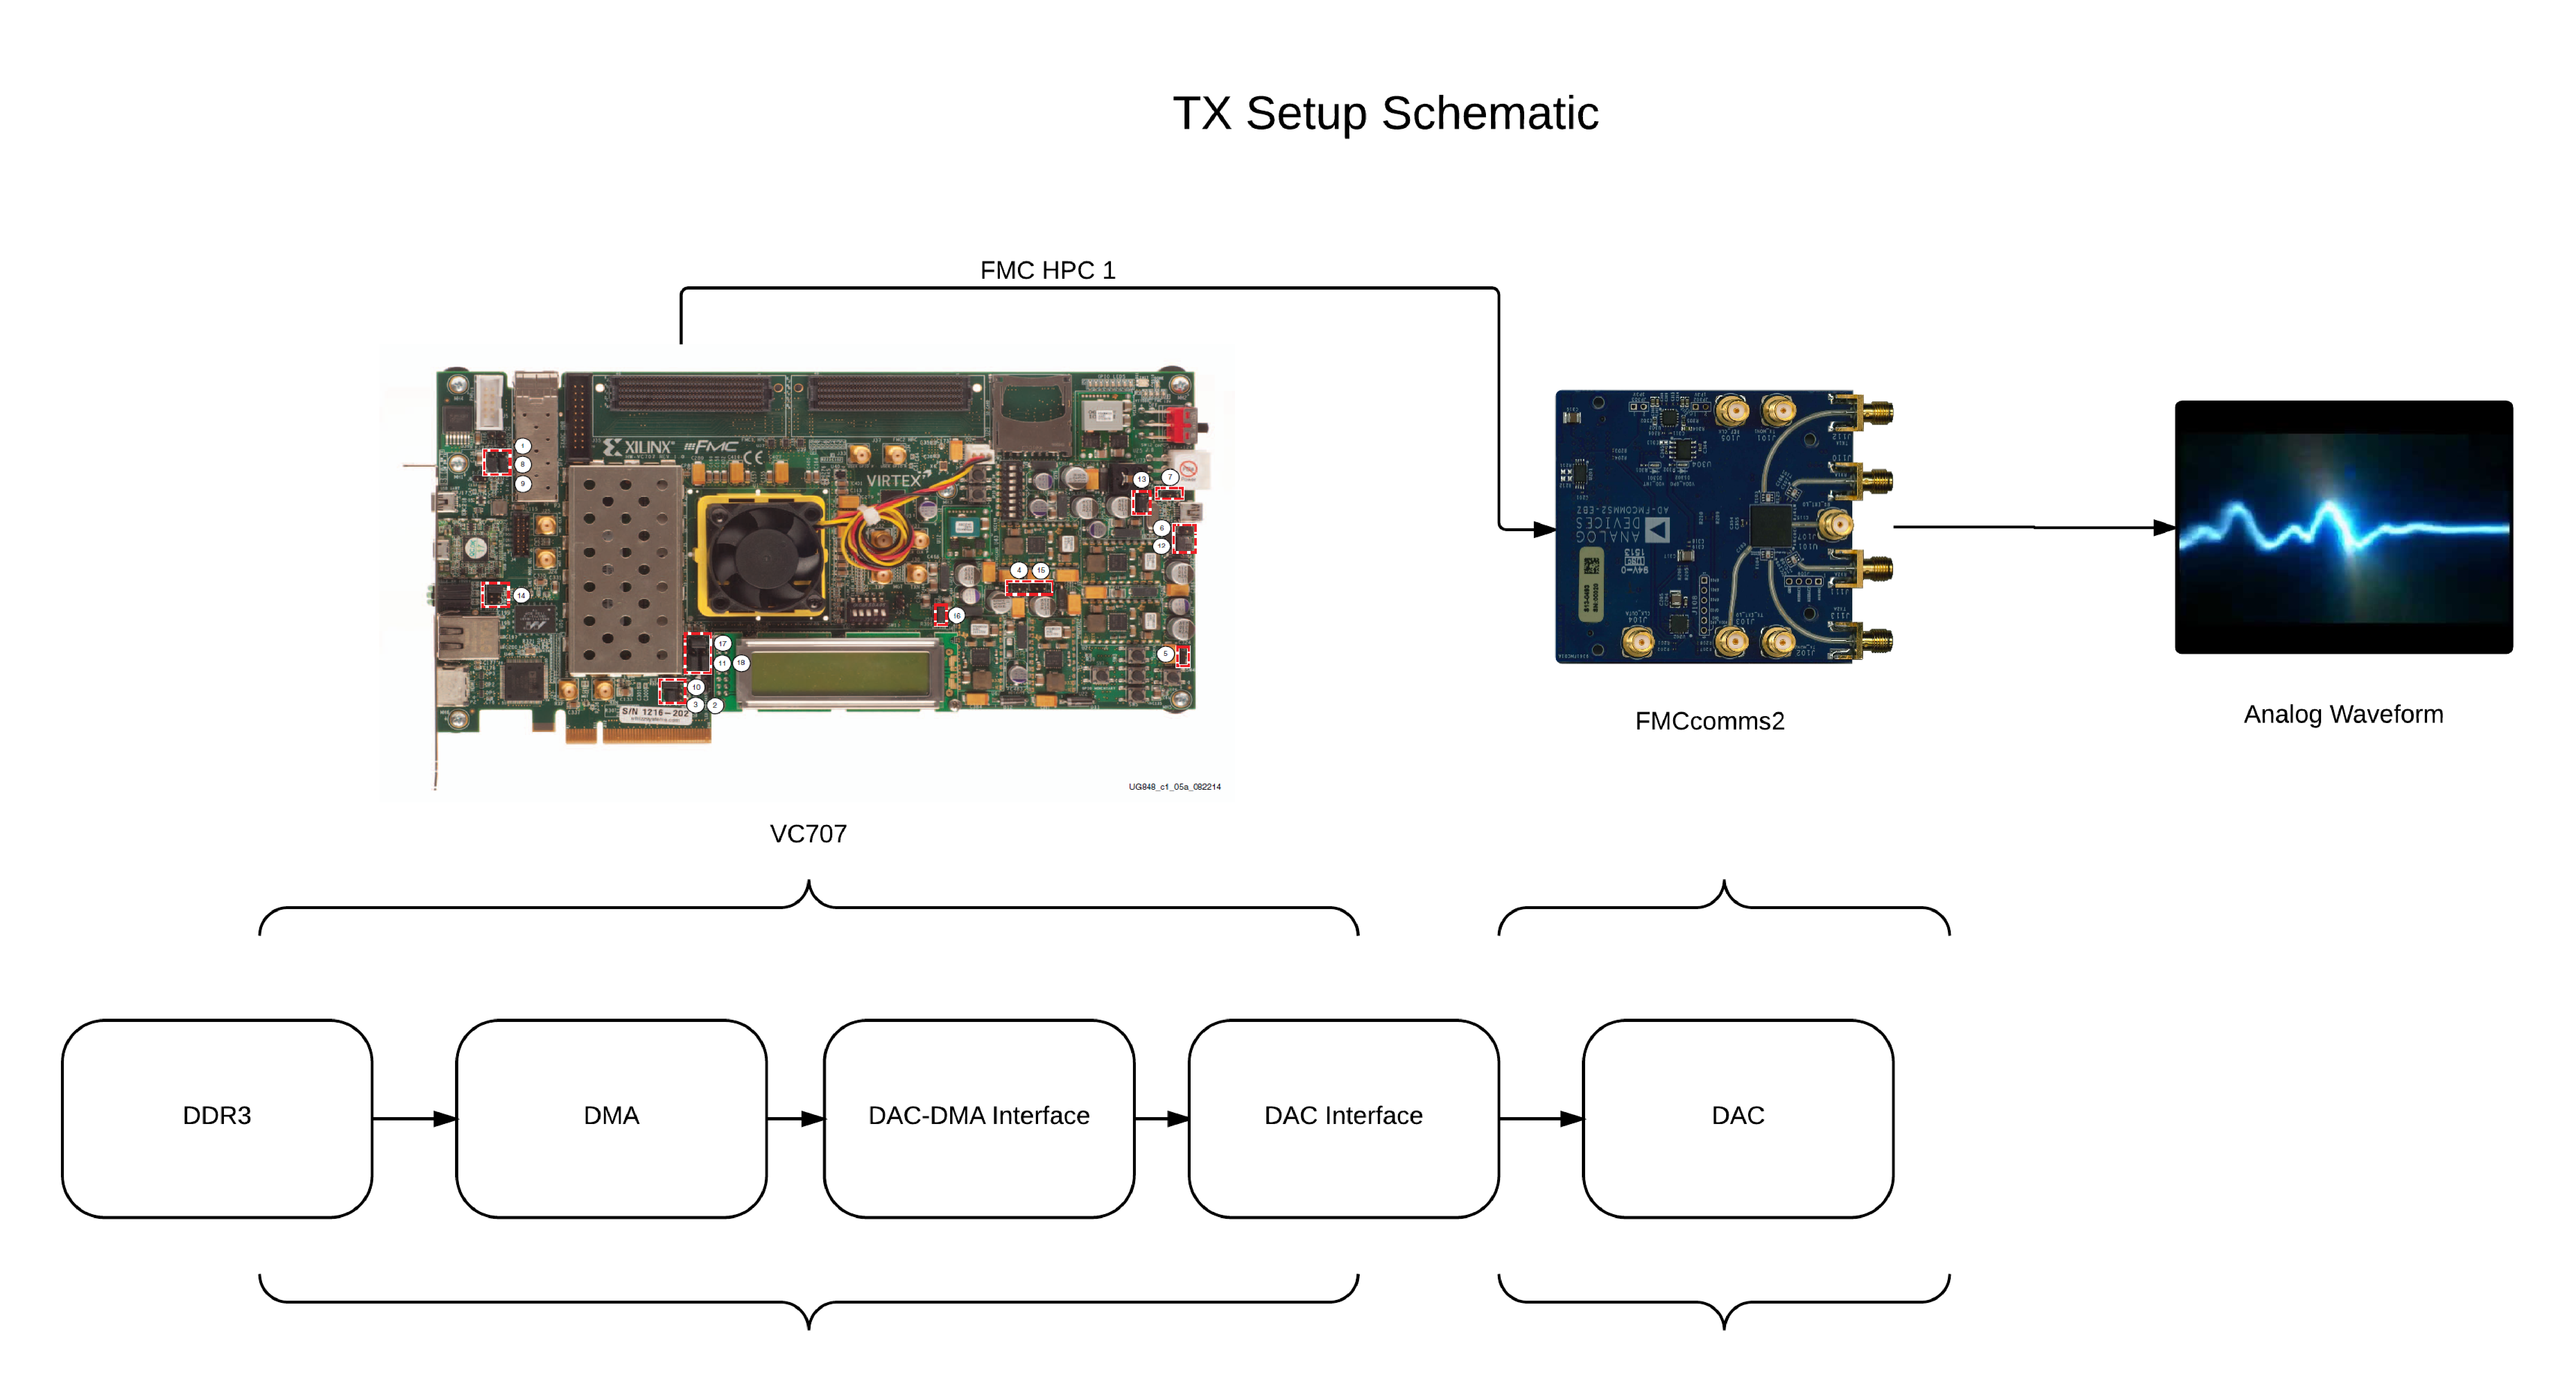
\includegraphics[width=0.9\textwidth]{./figures/tx_setup}
    \caption{ Transmitter setup block diagram.
    \label{fig:txsetup}}
%\end{figure}

%rx block diagram
%\begin{figure}[htbp]
    \centering
    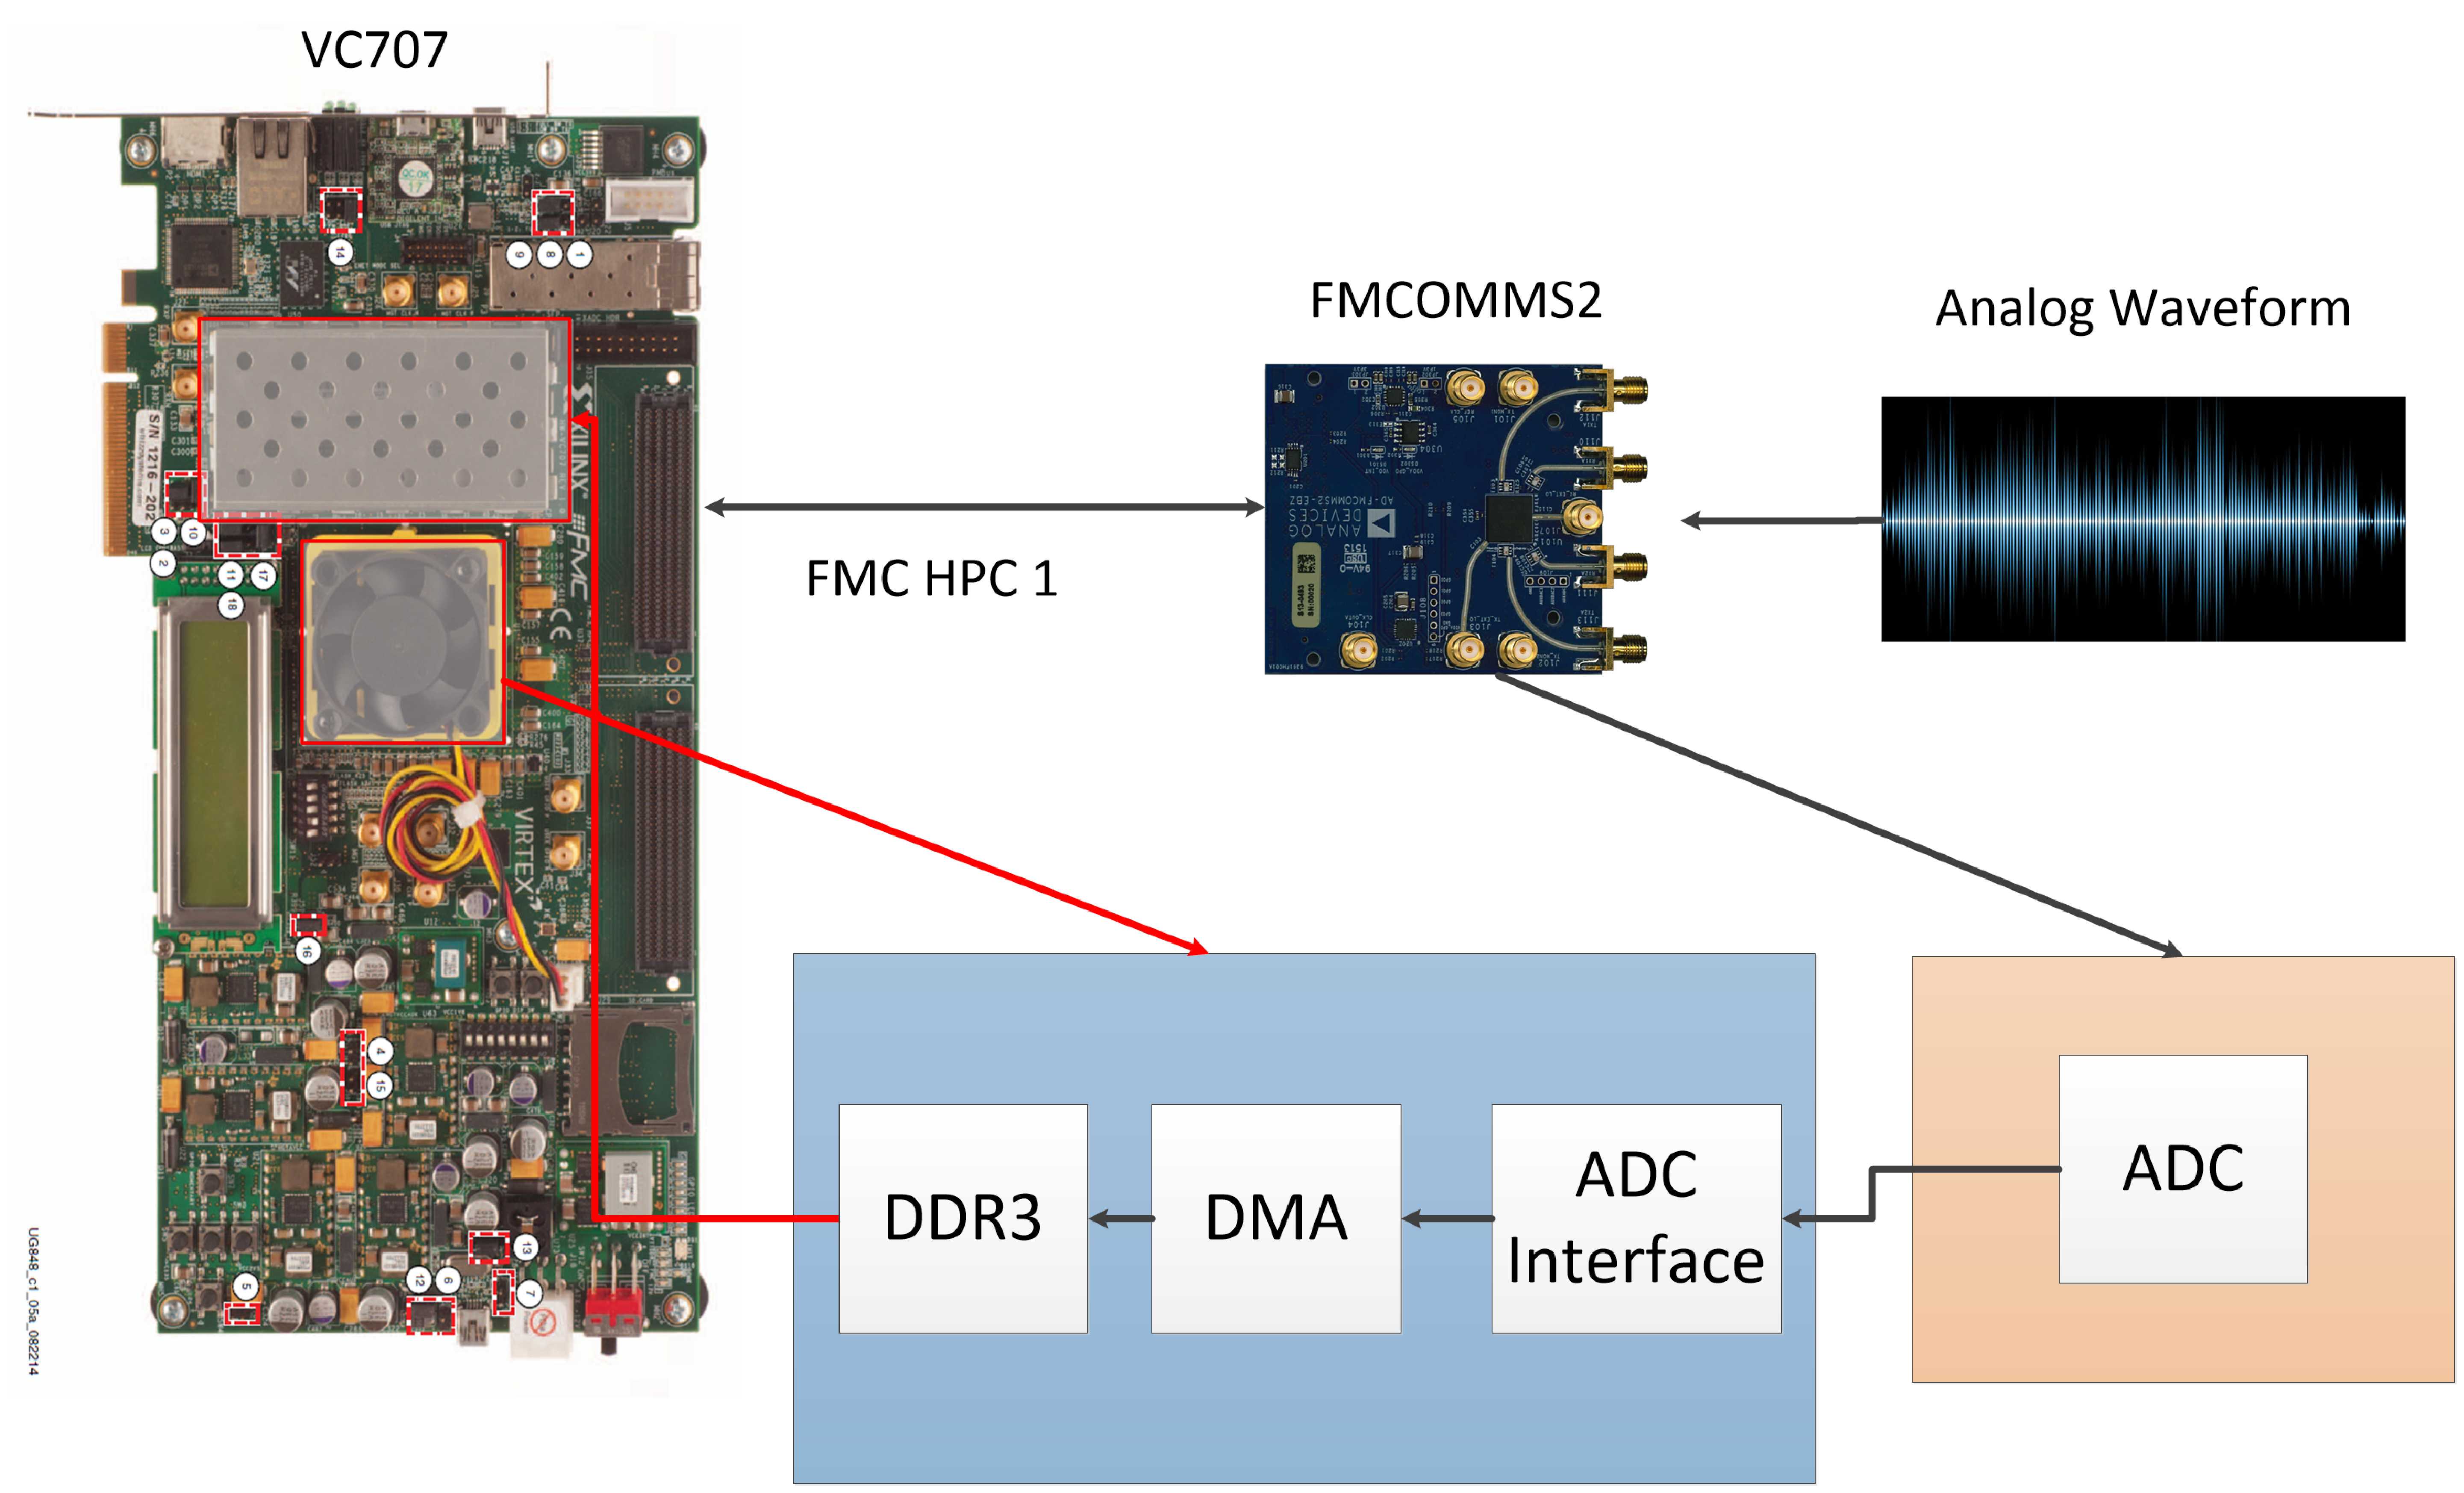
\includegraphics[width=0.9\textwidth]{./figures/rx_setup}
    \caption{ Receiver setup block diagram.
    \label{fig:rxsetup}}
\end{figure}



\subsection{Integration between FPGA and FMComms2}

The integration process was realized both in ML605 and VC707 because the latter
had a different development flow. For the development of the SDR prototype
presented in this work is to properly design the integration between the
FMComms2 and the FPGA. In order to accomplish this, the first steps involve the
analysis of the ports through which both communicate to each other and the
protocols in such communications. Additionally, it requires understanding about
the clocking supply that the AD9361 module in the FPGA requires. Finally, the
integration requires the designer to sufficiently understand the HDL sources of
the AD9361 IP core included in the FPGA and the corresponding drivers to be
included in the processor program.

By default the AD9361 driver has a waveform generator which feeds the DAC with
the necessary samples to generate a carrier wave at 2.4GHz, so if the
initialization works, it is possible to monitor in the oscilloscope or spectrum
analyzer a sinusoidal (carrier) wave at 2.4 GHz after all initialization
procedures have been concluded.

\subsection{Control Interface}
\label{subs:controlif}

As stated in the previous subsection, the FMCOMMS2 control and communication
interface is implemented through GPIO pins and an SPI communication between FPGA
and AD9361. SPI is used to write and read registers in the board while GPIO is
used for real-time control, like reset or change of states in the state machine
that governs AD9361 operation, the enable state machine (ENSM).

In order to facilitate and better organize the development through the IP
integrator in Vivado (were many IP cores are connected to each other), an IP
core was developed uniquely to handle the routing between the AD9361 IP
(supplied by Analog Devices) and the external GPIO and SPI ports. The IP was
named \emph{ad9361\_comm}.

In Figure \ref{fig:commif} it is possible to see in a simple schematic what is
the \emph{ad9361\_comm} IP and illustrates the routing of the respective ports
to the AD9361 interface. Where in the FPGA we have the SPI and GPIO IP cores
and they are routed by the \emph{ad9361\_comm} IP. The GPIO IP core in its
basic configuration has 3 basic ports, with variable bit length,  in this case
the length was 16. The \emph{ad9361\_comm} routes this pins with the
\emph{ad\_iobuf} block to match the AD9361 real-time control interface, but in
this work only the reset\_b pin is used. The SPI routing is simpler than the
GPIO, basically it unifies some input and output pins to create a in/out like
port and renames to match the AD9361 interface also.


%diagrama de blocos control interface
\begin{figure}[htbp]
    \centering
    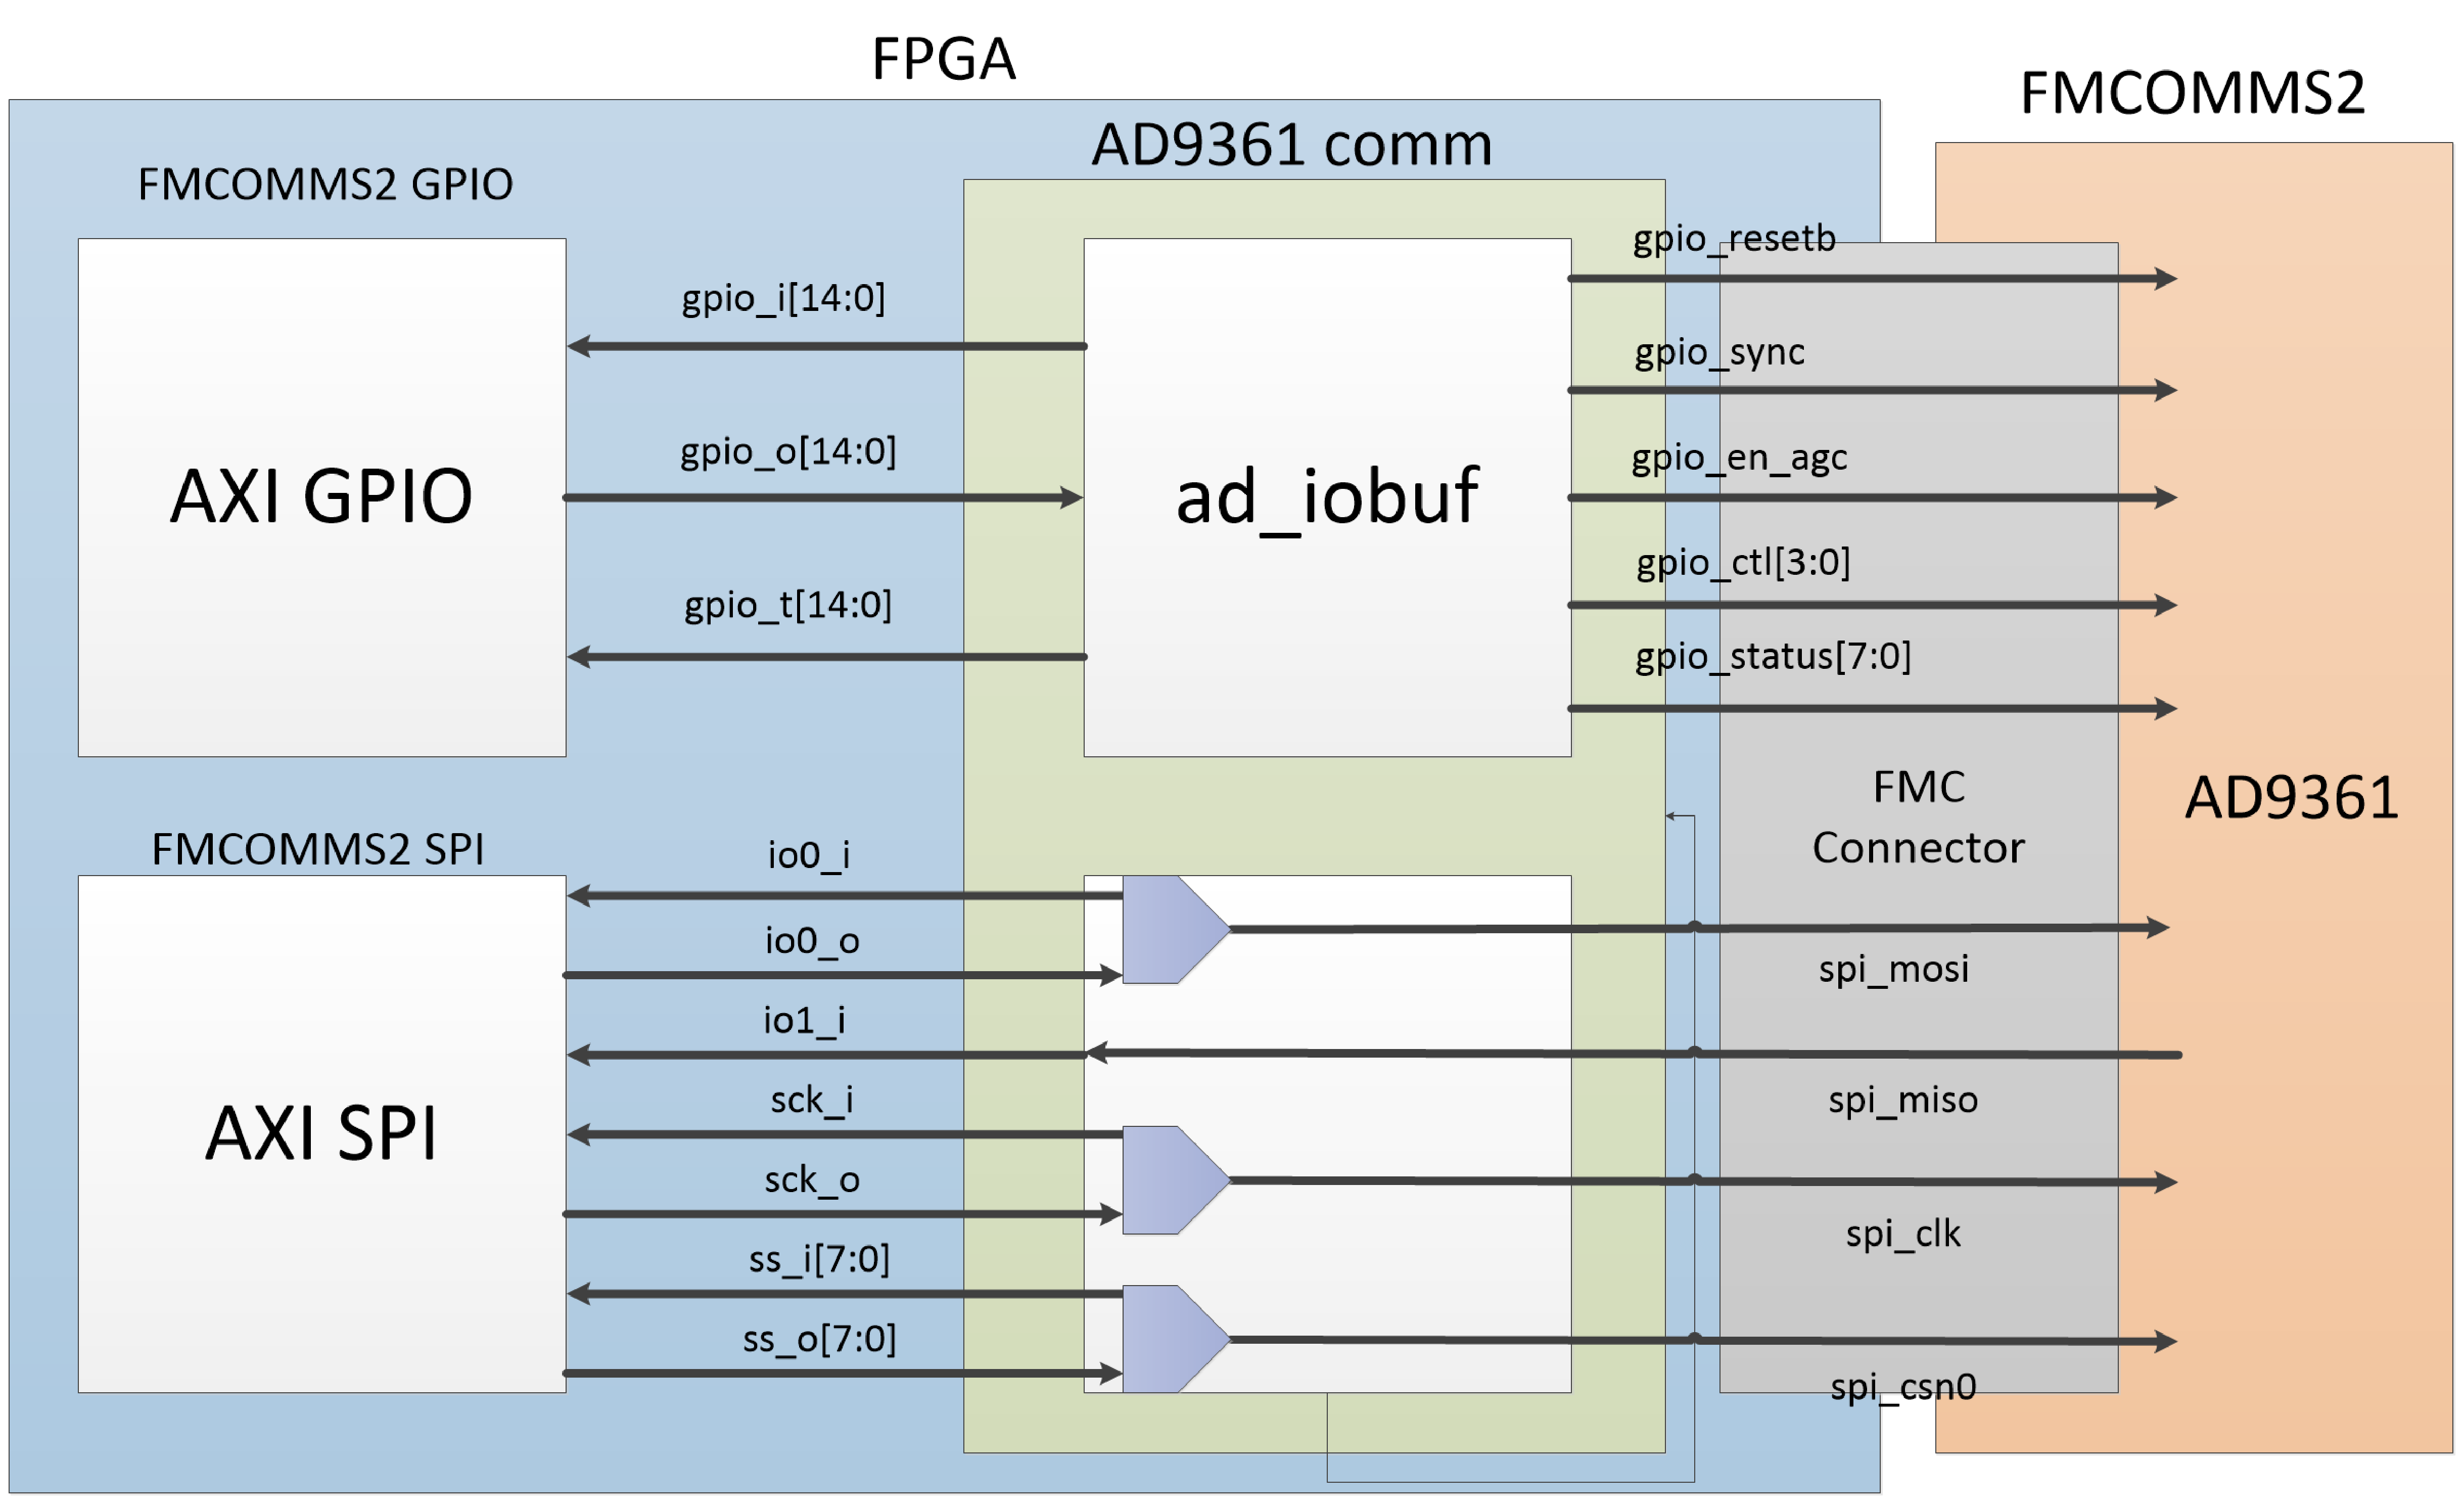
\includegraphics[width=0.9\textwidth]{./figures/comm_if}
    \caption{ Control interface block diagram.
    \label{fig:commif}}
\end{figure}

\subsection{Transmitting custom data}

Once communication and initialization between FPGA and FMCOMMS2 board works
properly, the next step is to input custom data into the device and efficiently
transmit modulated information in the carrier wave. Figure \ref{fig:txpins}
illustrates the transmitting data interface and shows that AD9361 works with IQ
data having one channel for I (16 bits) and one for Q (16 bits). It has also a
data flow control with the \emph{dac\_valid} and \emph{dac\_enable} ports in
each channel (I and Q). This data flow control is similar to the one implemented
in the AXI stream \cite{xilinx:axi} where the master and slave block exchange
signals in order to control this data flux. In the transmitter the AD9361 is the
master, so it reads data, then it should signal to the DMA or FIFO block that it
is ready to receive the data or not.

%inserir figura do IP AD9361 highlight TX interface pins
\begin{figure}[htbp]
    \centering
    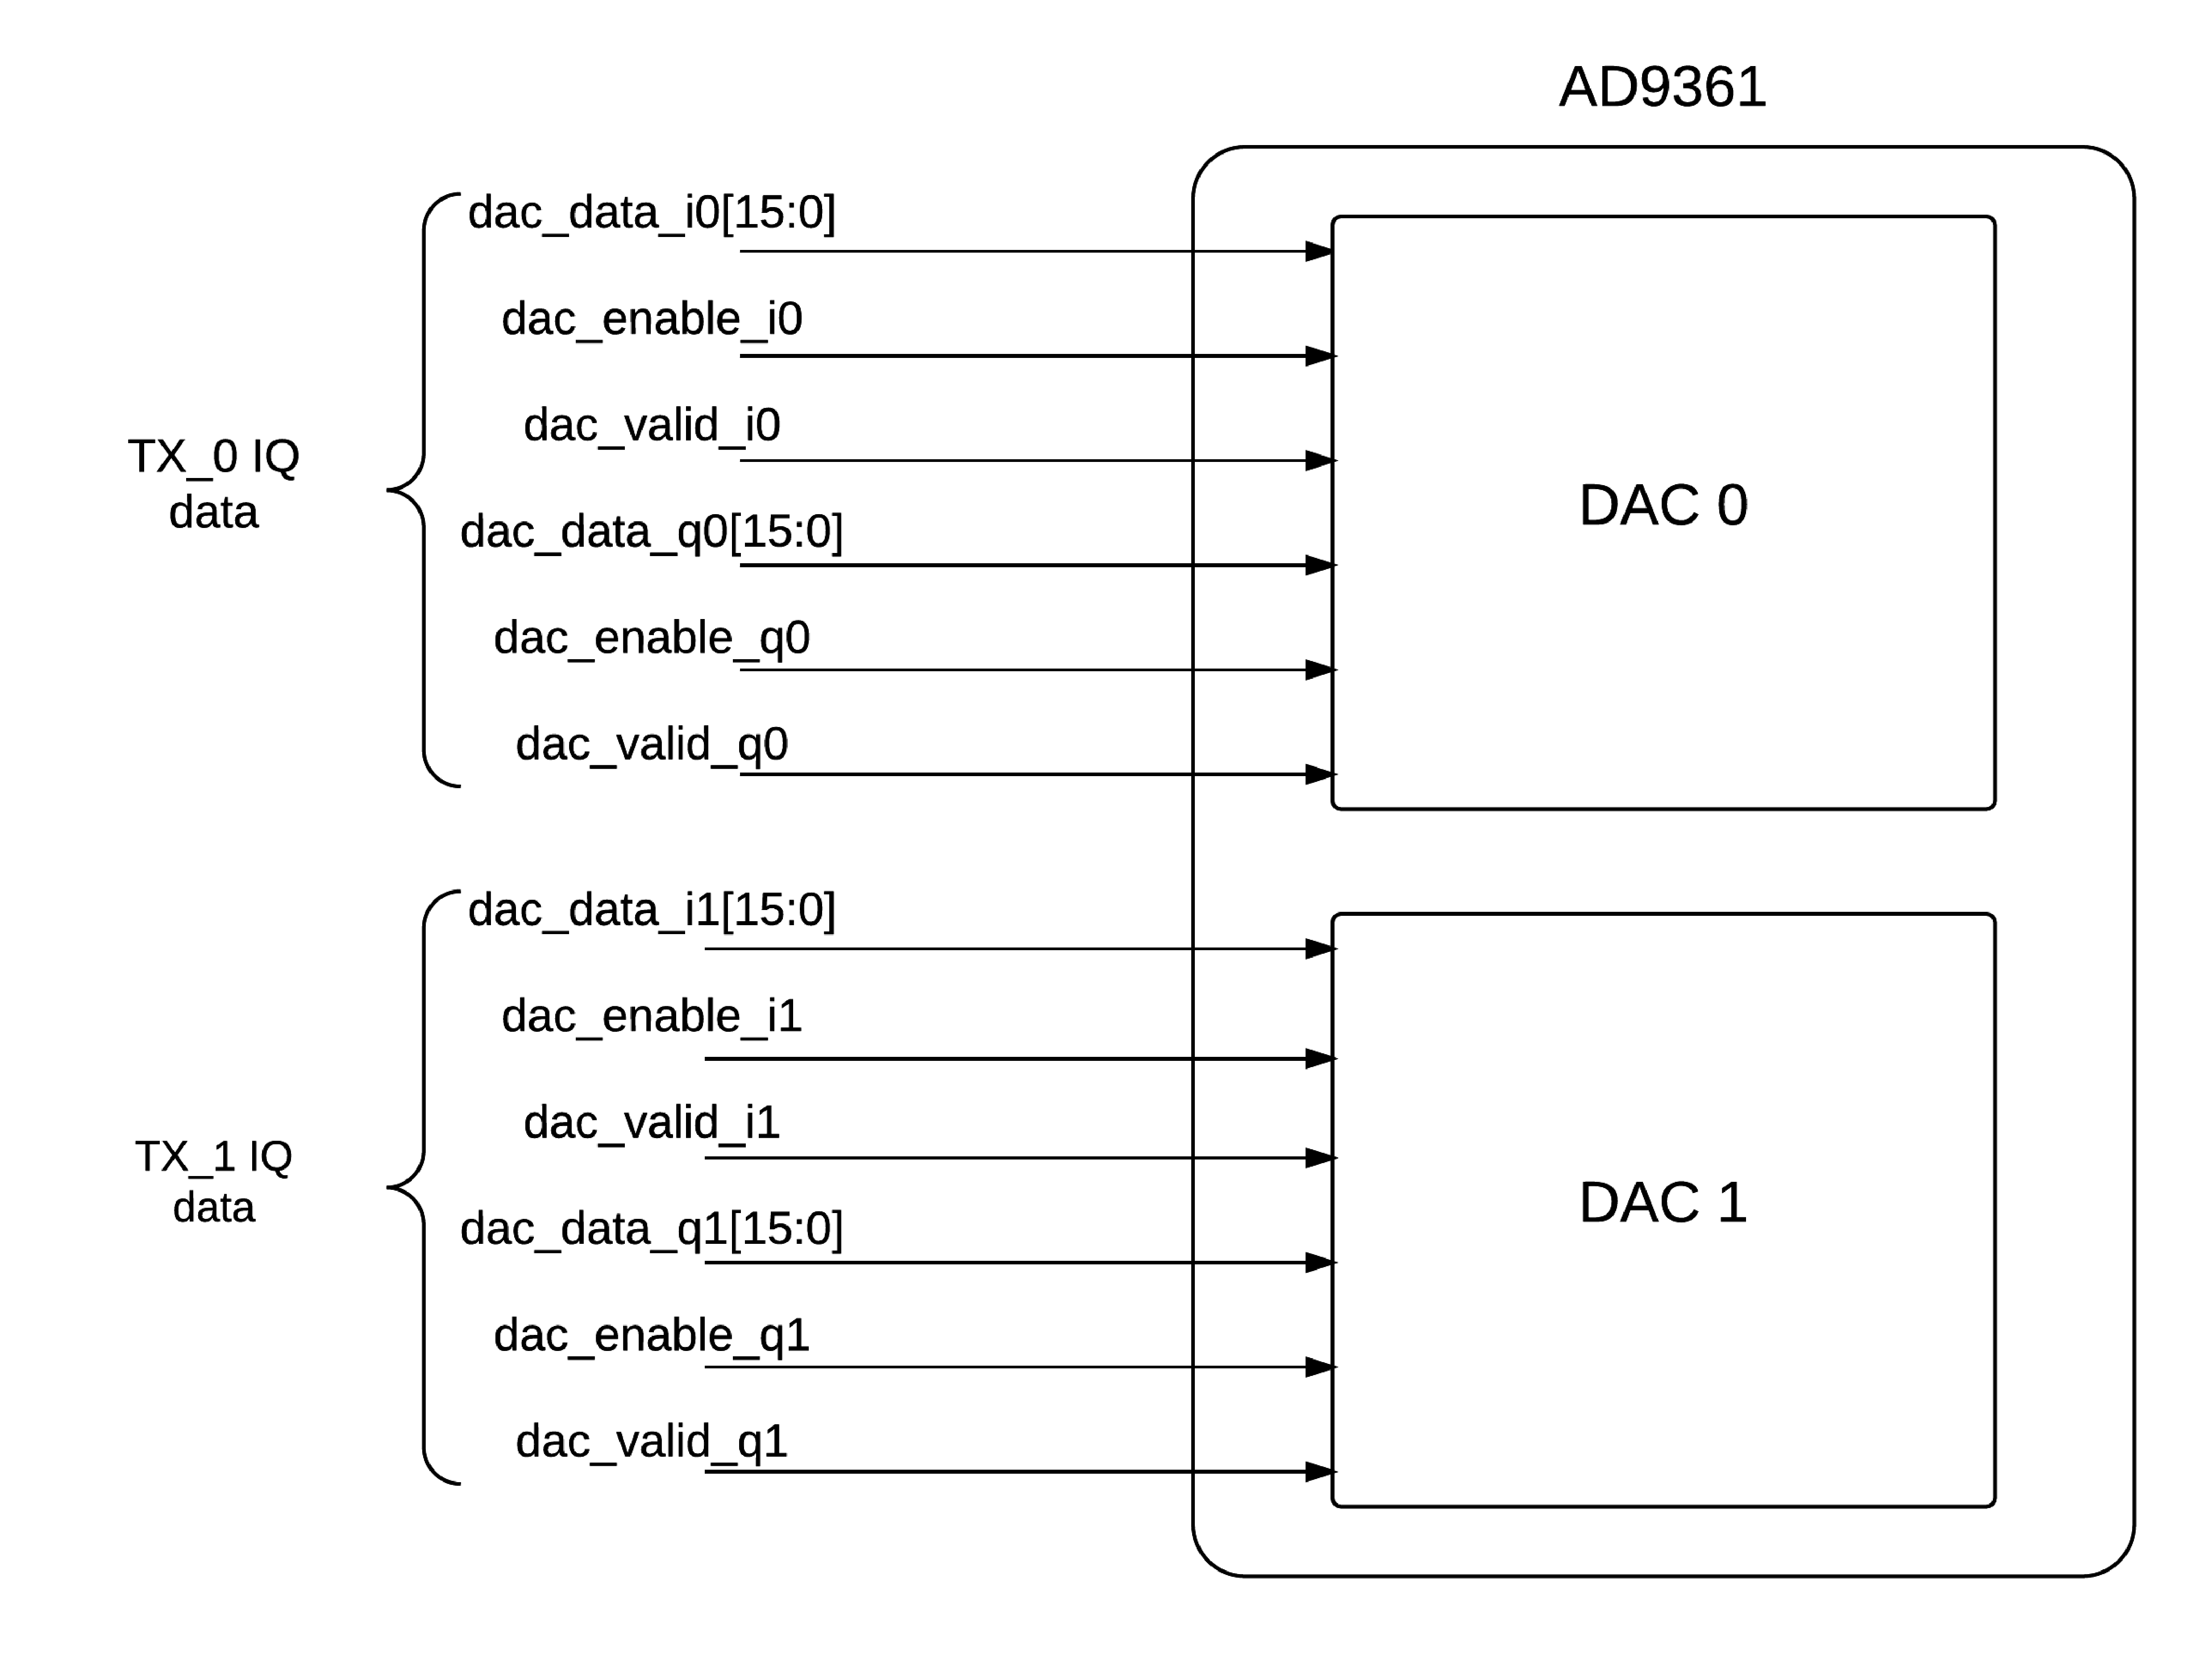
\includegraphics[width=0.605\textwidth]{./figures/ad9361tx_pins}
    \caption{ AD9361 transmitter (DAC) interface pins.
    \label{fig:txpins}}
\end{figure}

There are two ways to input data into the AD9361, the first one requires a
static data source (a signal generator was used in this work) feeding a FIFO
connected directly to the AD9361 data ports and the second solution aims to
replace such "static data source" for a dynamic and software controlled data
source, accomplished by the use of DMA. Figure \ref{fig:ad9361txfifo} shows a
scheme that illustrates the first method. Note that are no proper flow control
implemented. However, this method is slow and can lose data easily because the
DAC clock is inferior to the FPGA signal generation clock, which implies that
DAC cannot read as fast as the FPGA can generate. In contrast, the DMA method
allows faster reading speed and better flow control. Figure
\ref{fig:ad9361txdma} illustrates this second alternative. Note that in this
figure there is the need of a data interface in order to distribute the memory
reading data (DDR3 - DMA) through the AD9361 data interface properly using only
one DMA IP core. With this block the 32 bits read at each cycle by the DMA are
simultaneous connected to the 32 bits IQ data interface ( 16 bits for I channel
and 16 bits for Q channel), that is, the 32 read bits go through the ADC 0 and
ADC 1 simultaneously.

%inserir diagrama de blocos de entrada DDS>FIFO>AD9361

\begin{figure}[htbp]
    \centering
    
\includegraphics[width=0.85\textwidth]{./figures/dac_fifo}
    \caption{ AD9361 DAC interface with FIFO.
    \label{fig:ad9361txfifo}}
\end{figure}


%inserir figura da interface DMA>AD9361
\begin{figure}[htbp]
    \centering
    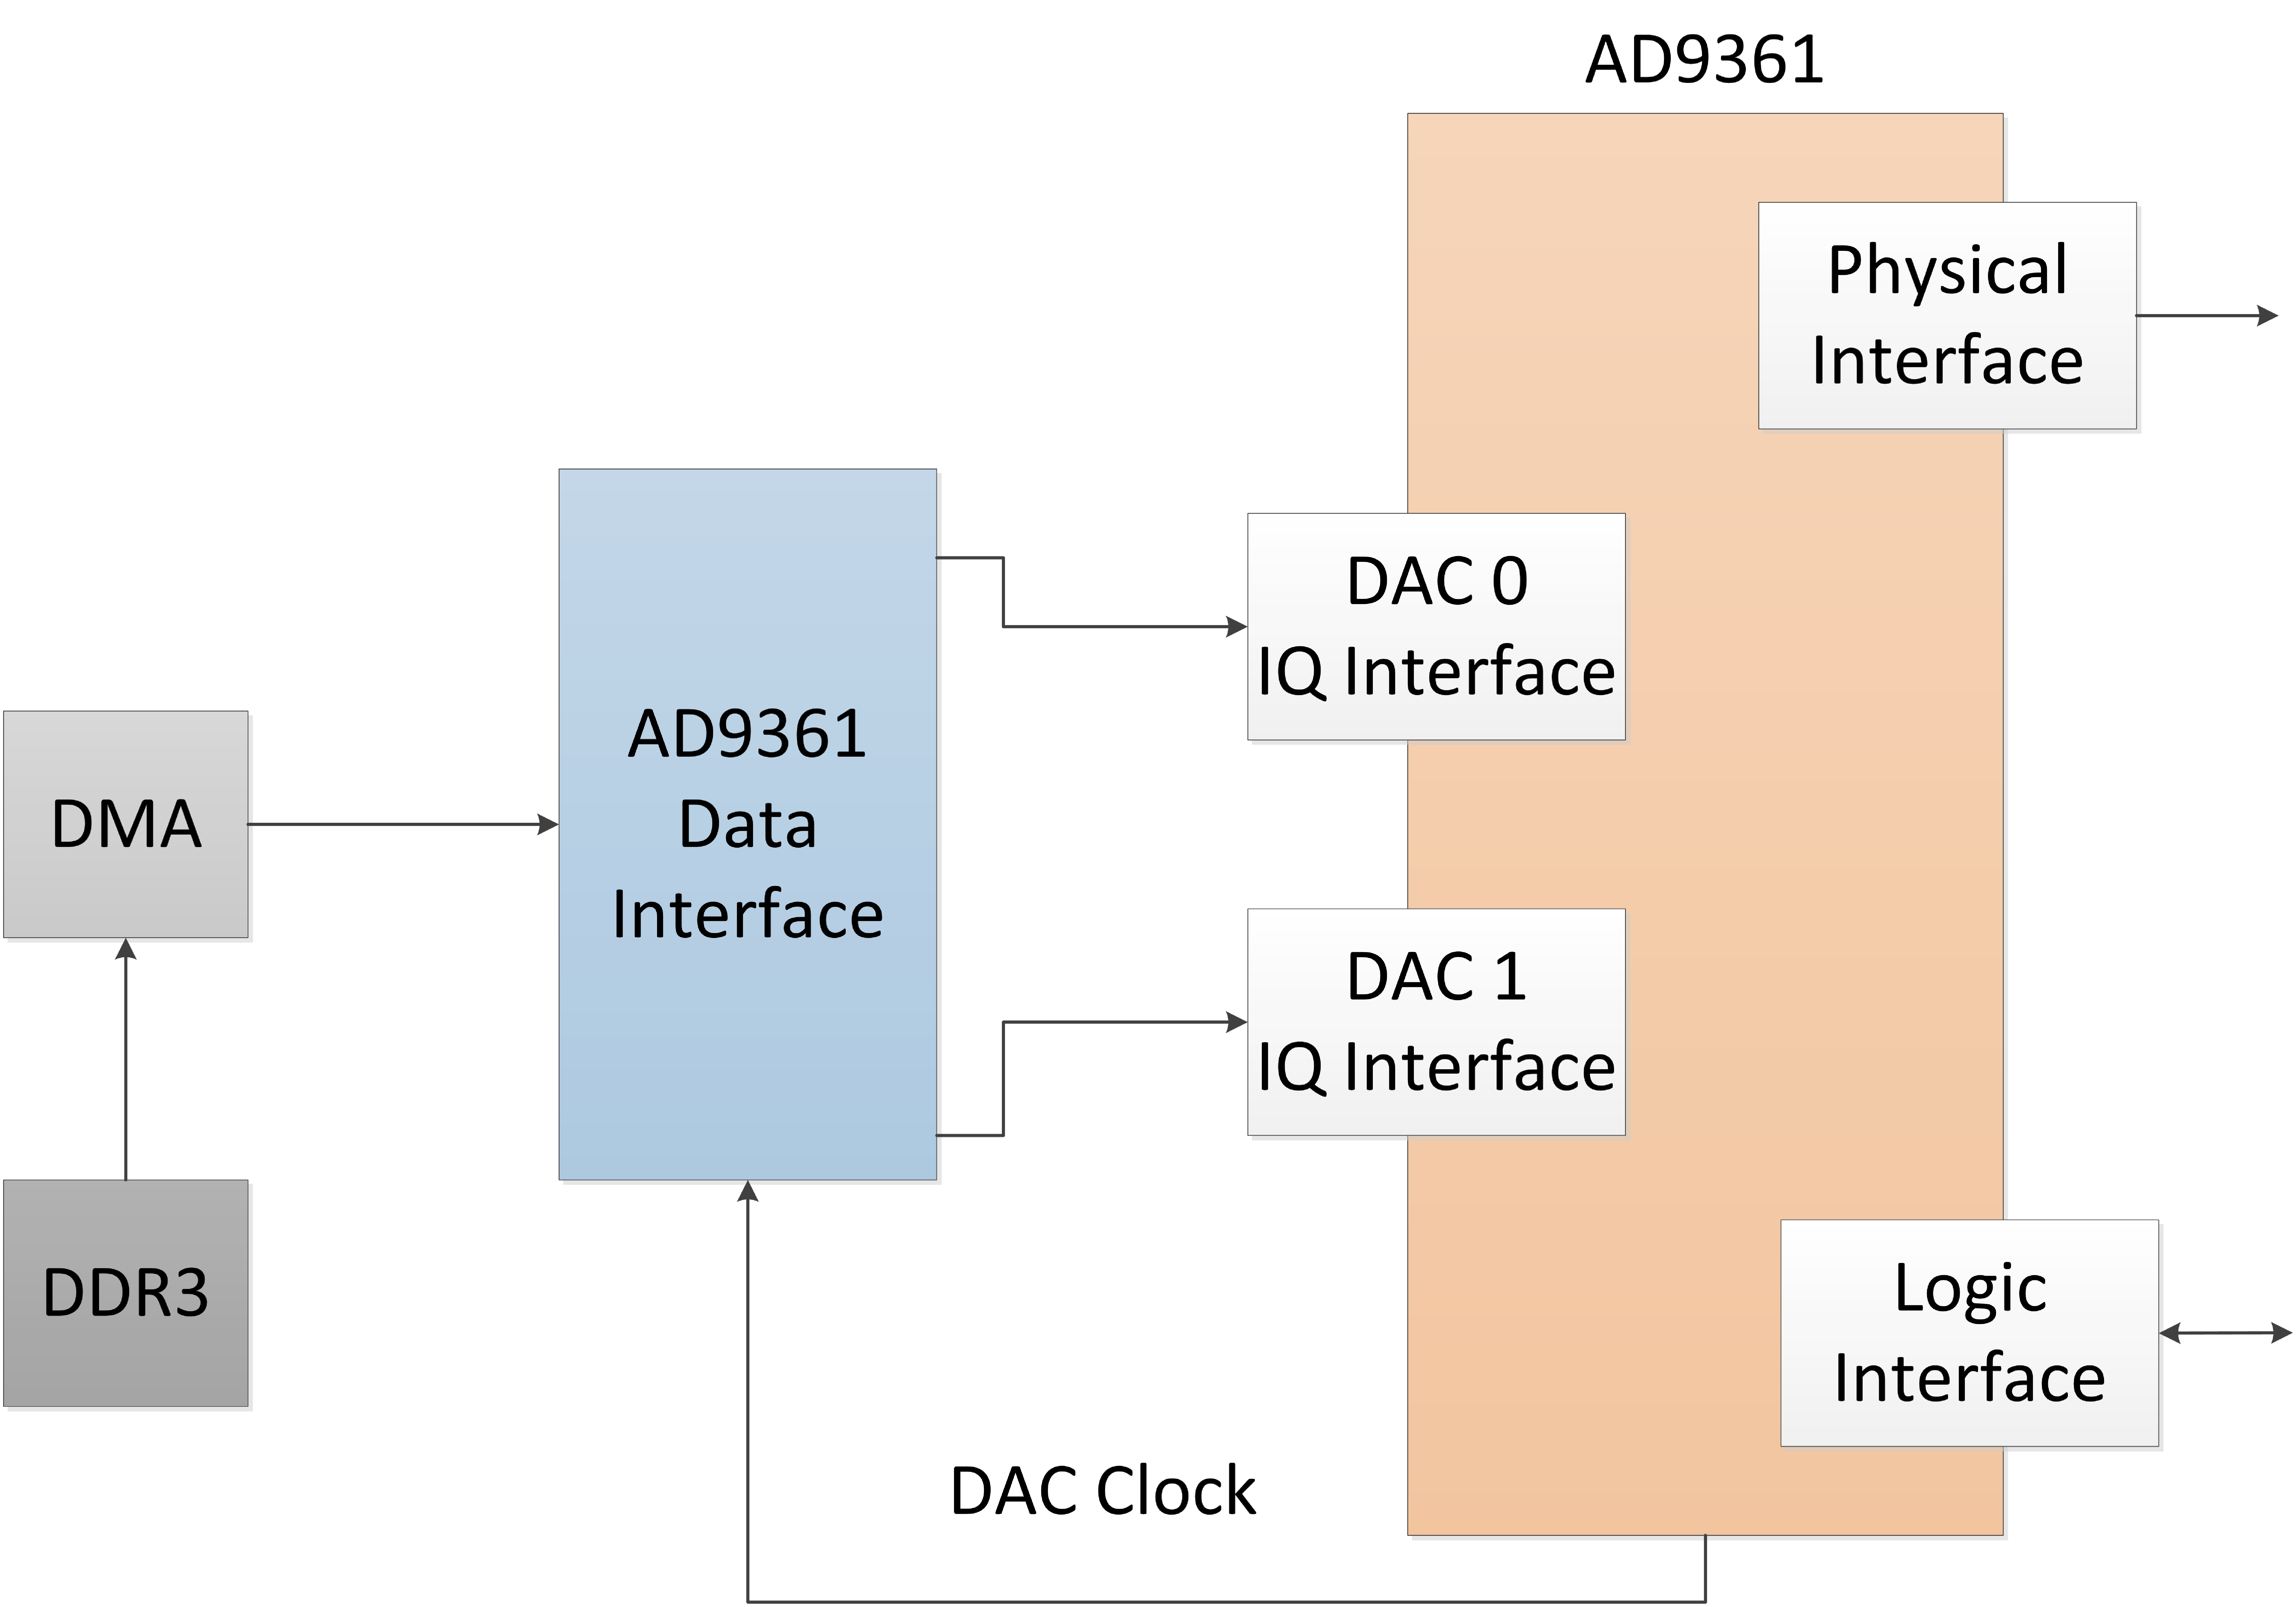
\includegraphics[width=0.85\textwidth]{./figures/dac_dma}
    \caption{ AD9361 DAC interface with DMA.
    \label{fig:ad9361txdma}}
\end{figure}

\vspace{50pt}

\subsection{Receiving Custom data}

Receiving is practically the opposite of transmitting custom data. Figure
\ref{fig:rxpins} illustrates the receiving data interface with the I and Q
channels and its respective \emph{valid} and \emph{enable} ports for flow
control. This interface acts in the same way as the receiving interface,
signaling when the bits can be read from the ADC.

%inserir figura do IP AD9361 Highlight RX interface pins
\begin{figure}[htbp]
    \centering
    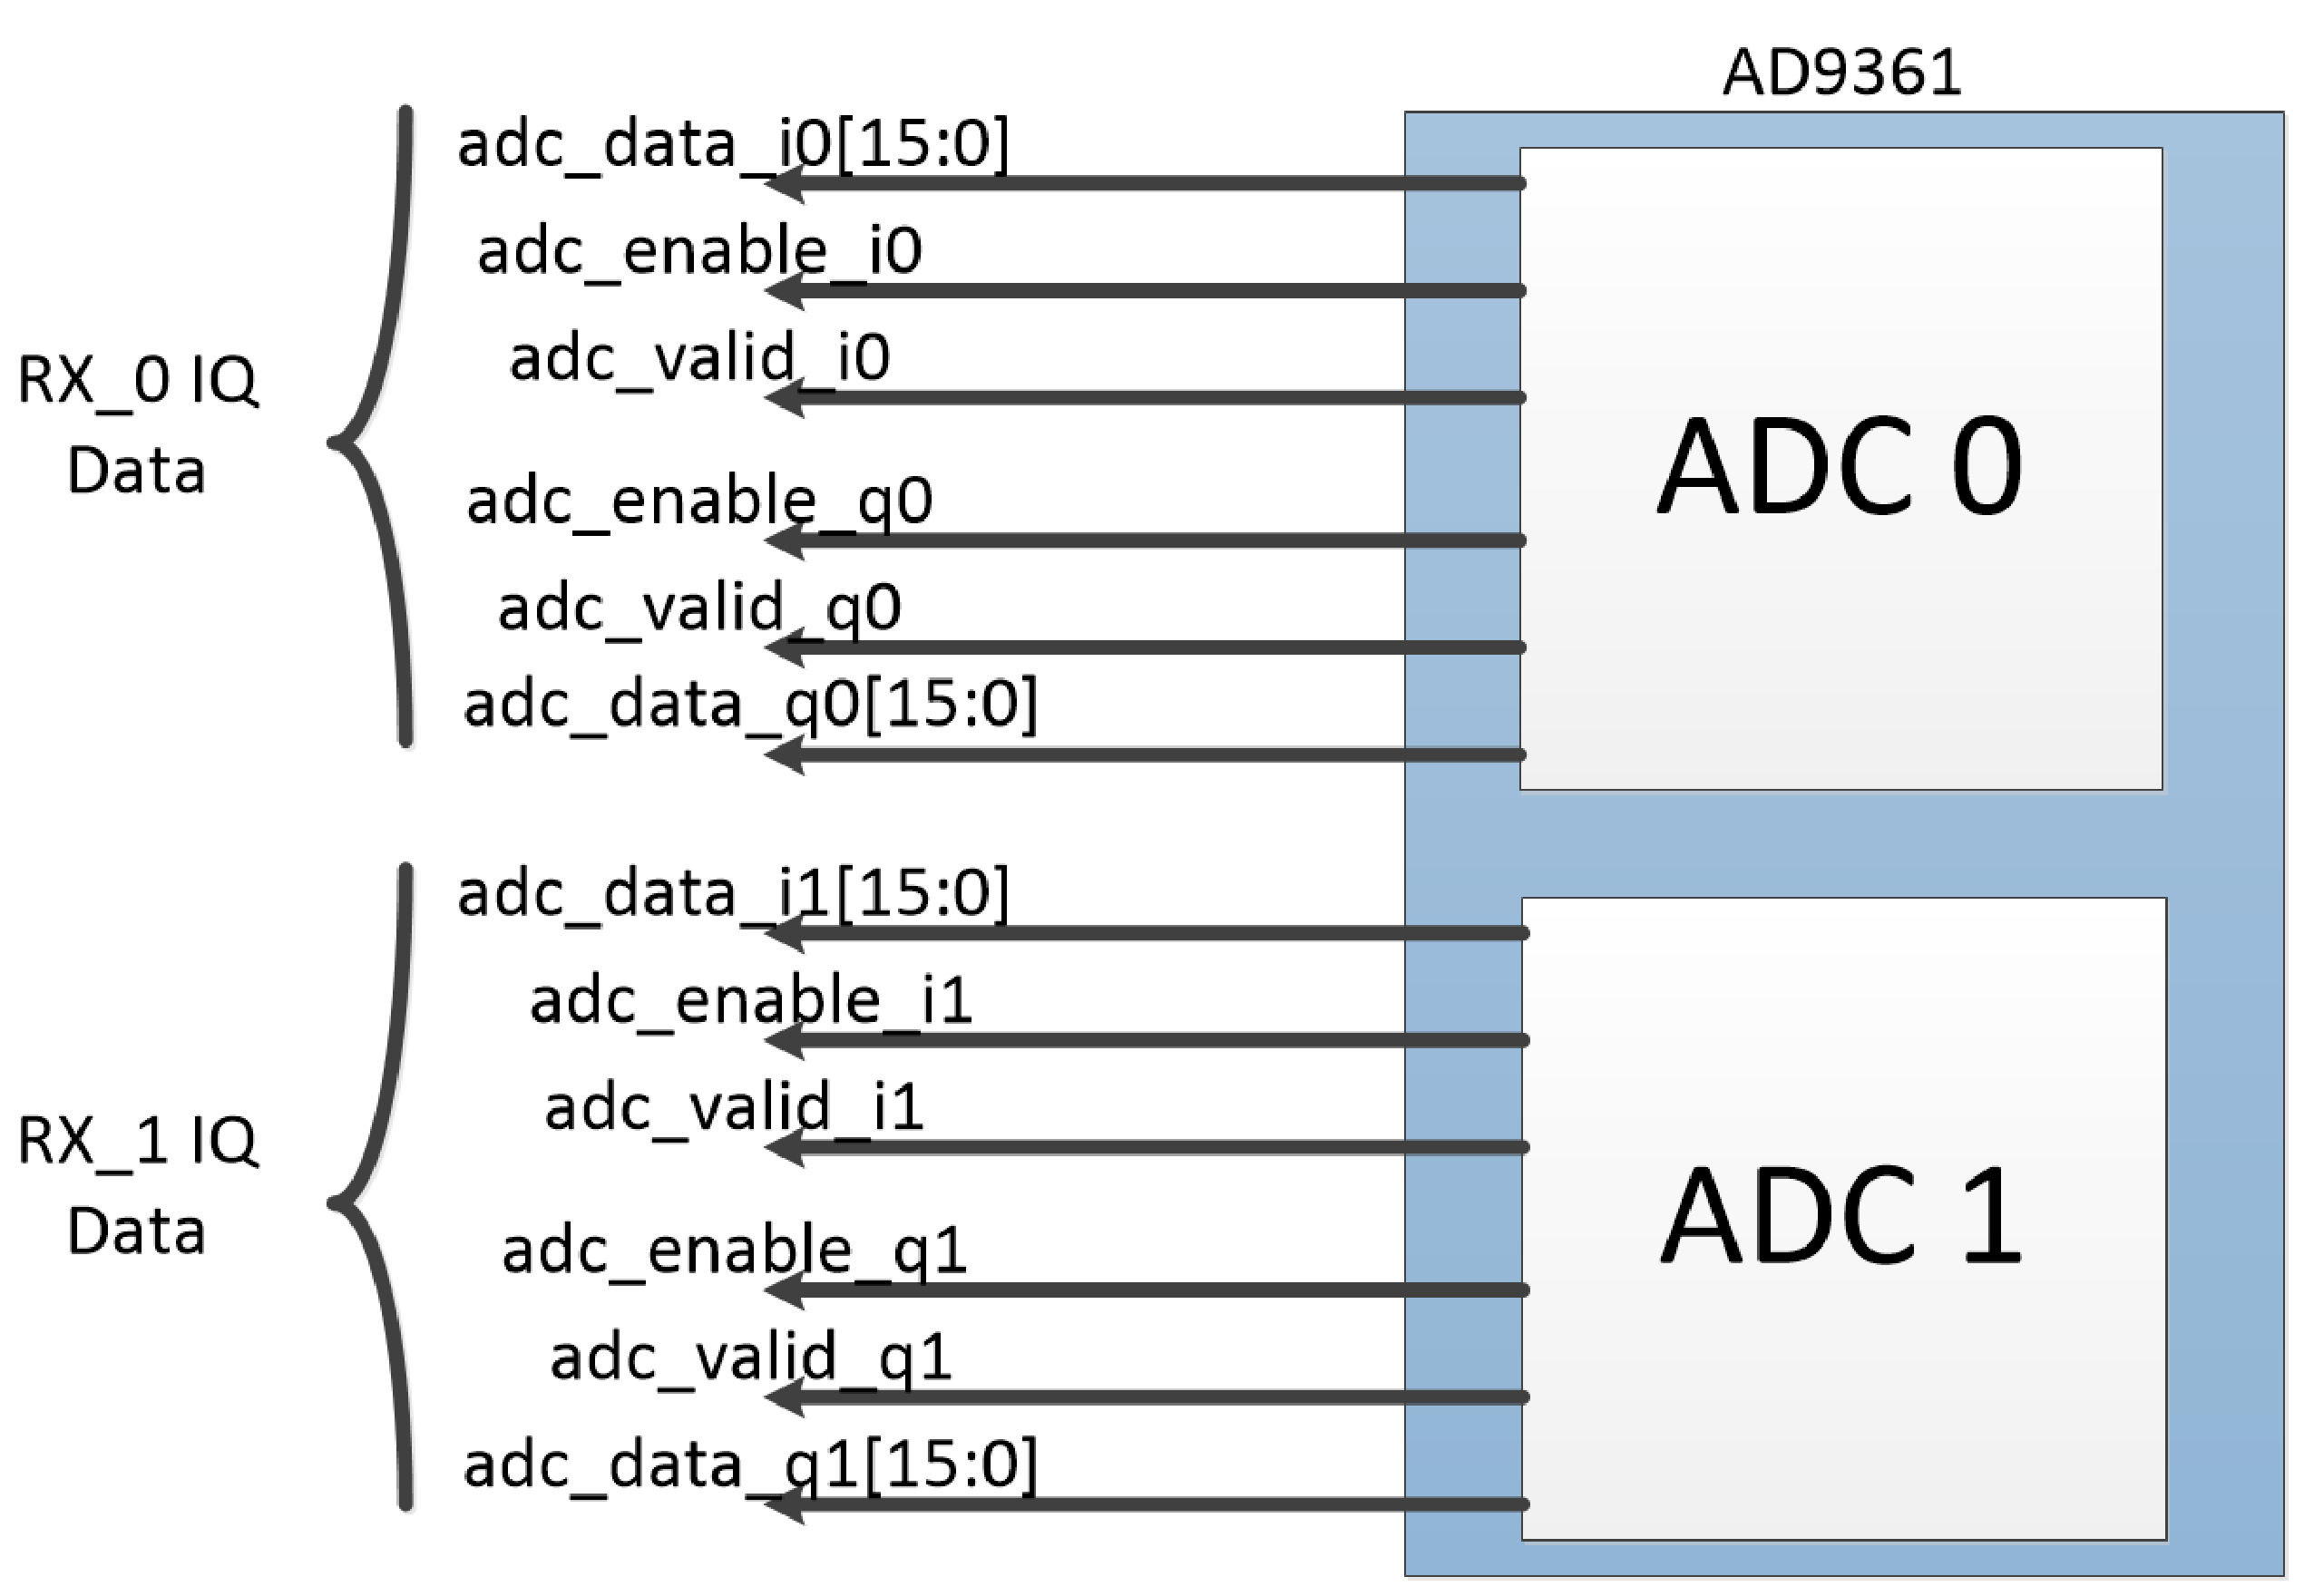
\includegraphics[width=0.6\textwidth]{./figures/ad9361rx_pins}
    \caption{ AD9361 receiver (ADC) interface pins.
    \label{fig:rxpins}}
\end{figure}

The same idea of the transmission is implemented in the reception with some
changes. Having two possible solutions, the first one being a simpler FIFO
interface that receives data from the ADC and sends it to a FPGA internal signal
debugging in Vivado Software and the second solution involves a more dynamic
approach, using the DMA to write the ADC output data to the memory allows such
data to be processed after reception like comparing to the transmitted data for
example. The Figure \ref{fig:ad9361rxfifo} illustrates the first solution. Note
that this approach is straight forward and simple. The second approach is
illustrated in Figure \ref{fig:ad9361rxdma} where like the transmitting
interface, it needs a data interface to multiplex the 64 bits received by both
channels in 32 bits segments that DMA can write in memory.


%inserir diagrama de blocos de entrada AD9361>FIFO>ILA
\begin{figure}[htbp]
    \centering
    
\includegraphics[width=0.85\textwidth]{./figures/adc_fifo}
    \caption{ AD9361 ADC interface with FIFO.
    \label{fig:ad9361rxfifo}}
\end{figure}

%inserir figura da interface AD9361>DMA
\begin{figure}[htbp]
    \centering
    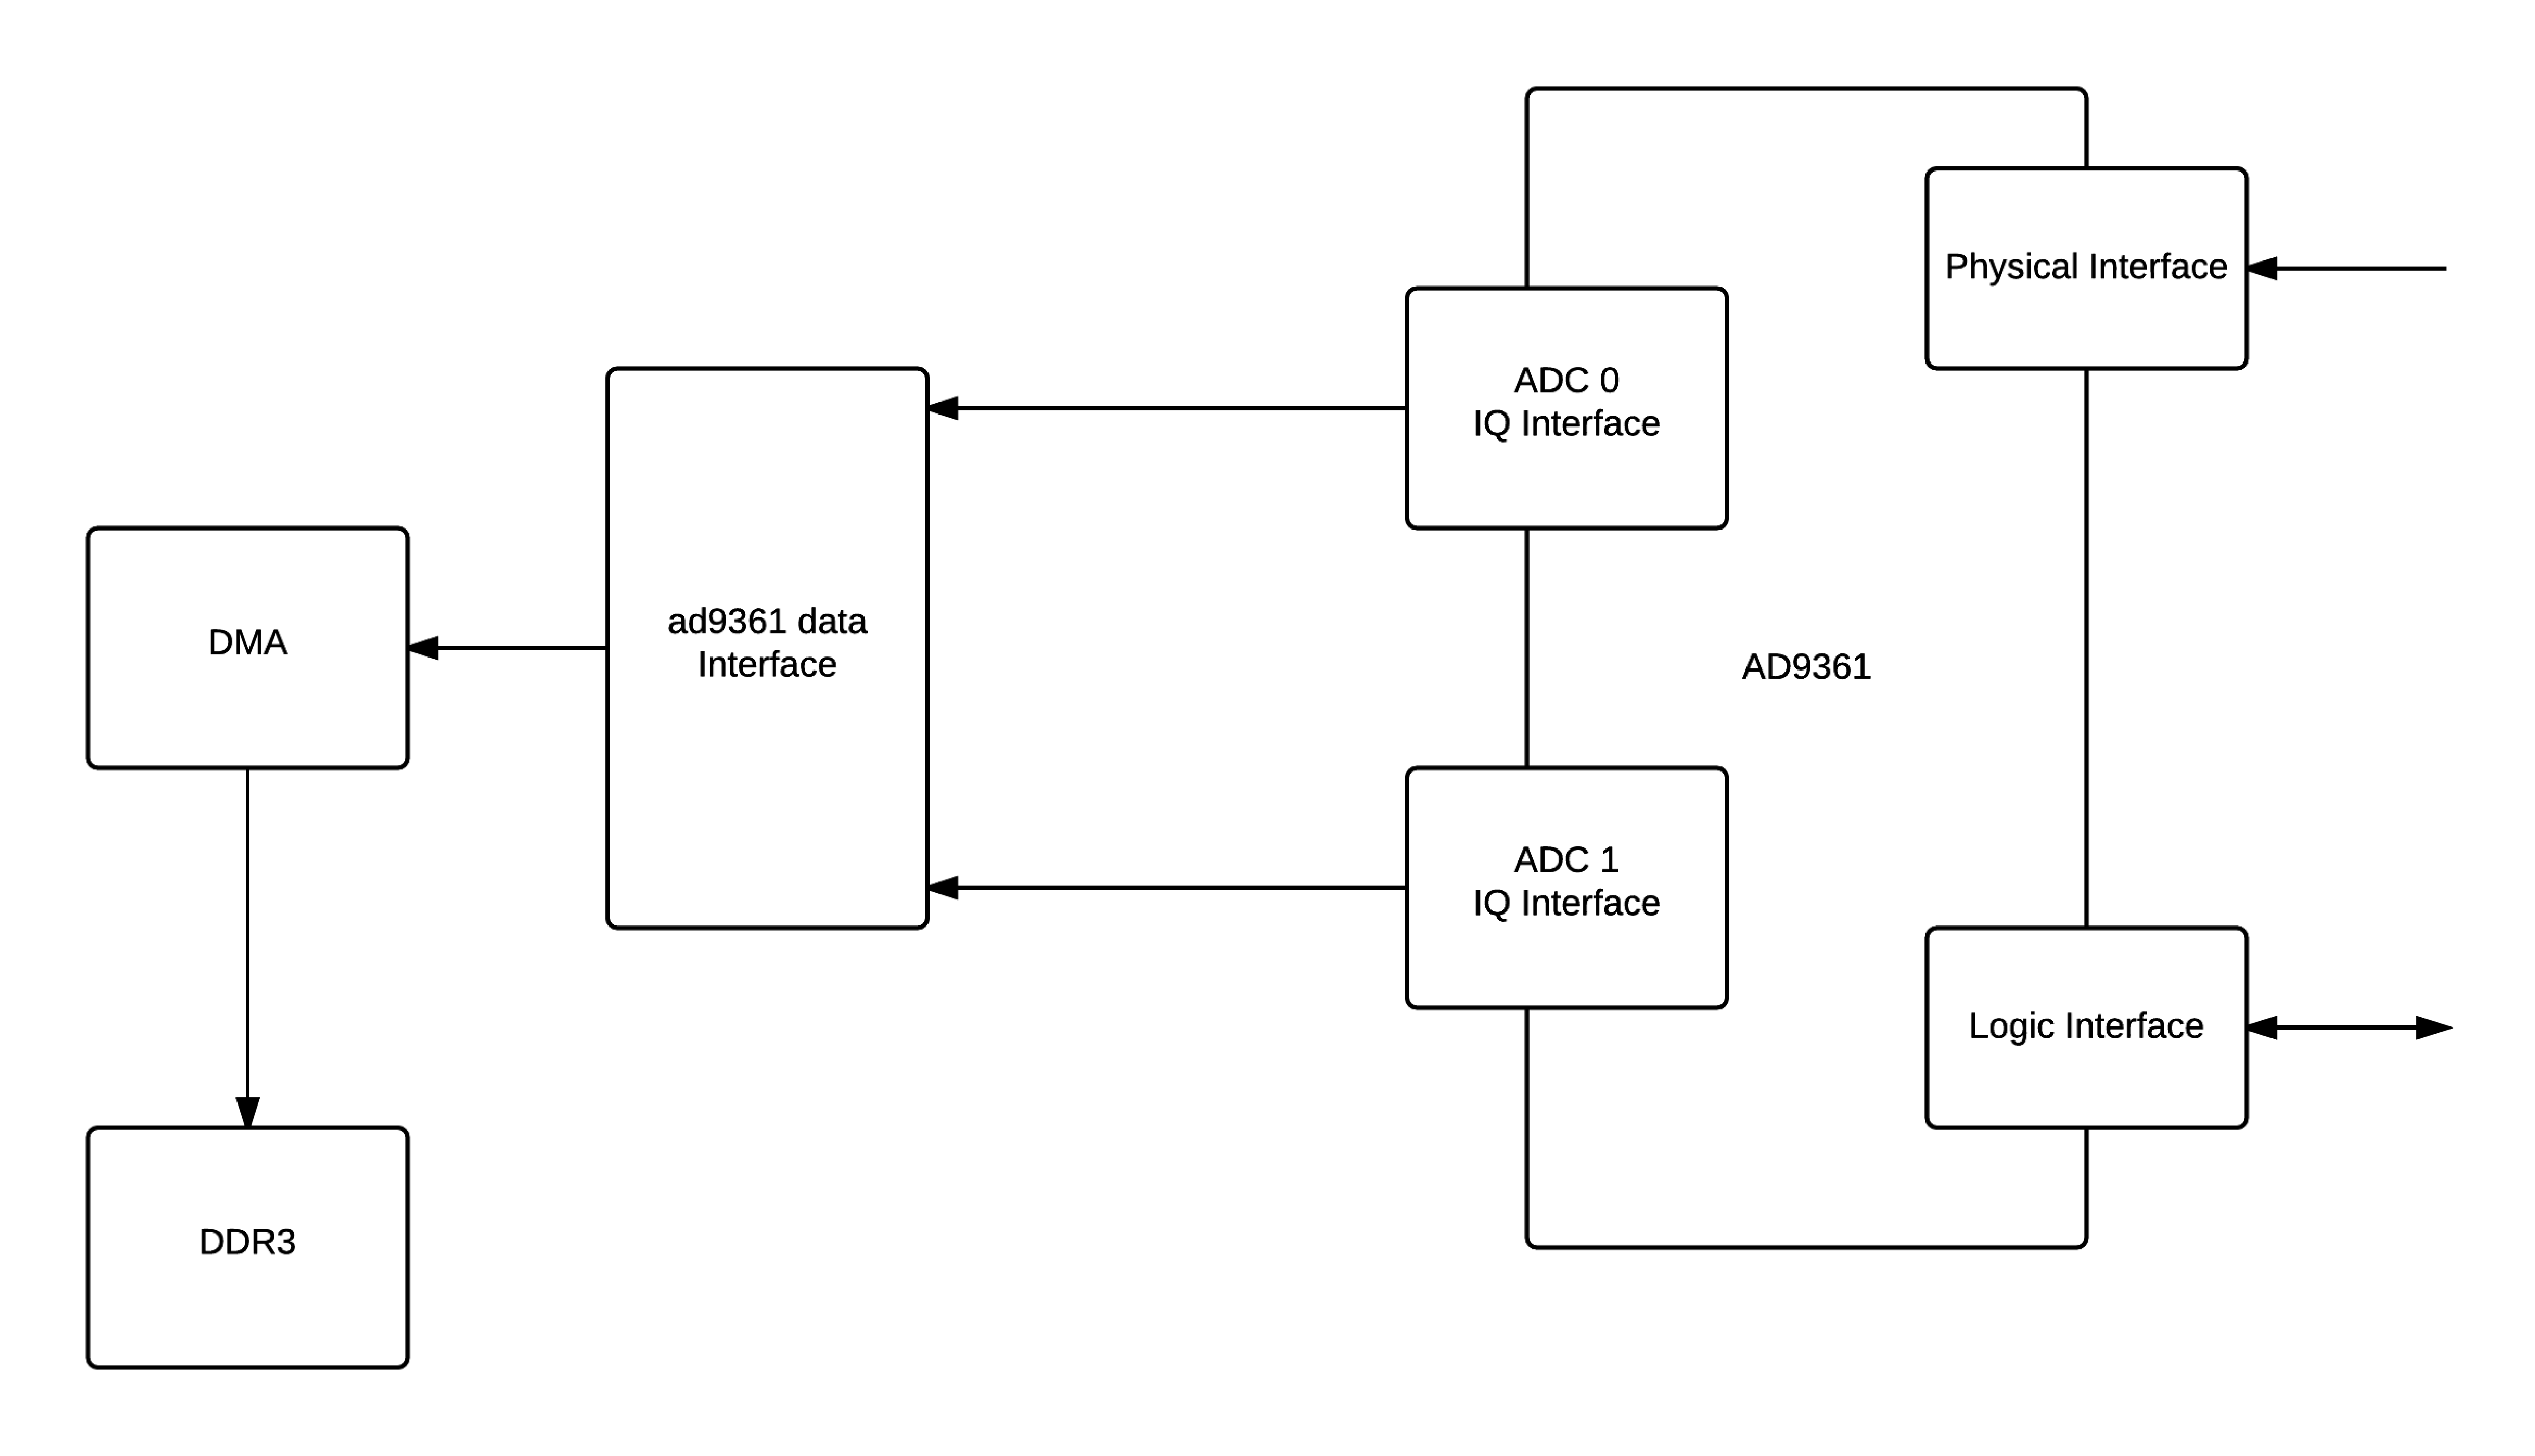
\includegraphics[width=0.85\textwidth]{./figures/adc_dma}
    \caption{ AD9361 ADC interface with DMA.
    \label{fig:ad9361rxdma}}
\end{figure}

\clearpage

\subsection{Data Interface}
\label{subs:dataif}

The data interface from the AD9361 to the FPGA logic is implemented as an IP in
the FPGA design named \emph{ad9361\_data} and is composed by two parts, a
transmitting interface and a receiving interface. A high level block diagram of
the data interface can be seen in Figure \ref{fig:databd}. The transmitting
interface connects the DMA, which is reading data from the main memory, with the
DAC interface and the receiving interface connects the ADC output with the DMA
that writes on the main memory, in the subsections below the two interfaces will
be explained in more detail.

%ad9361_data interface image
\begin{figure}[htbp]
    \centering
    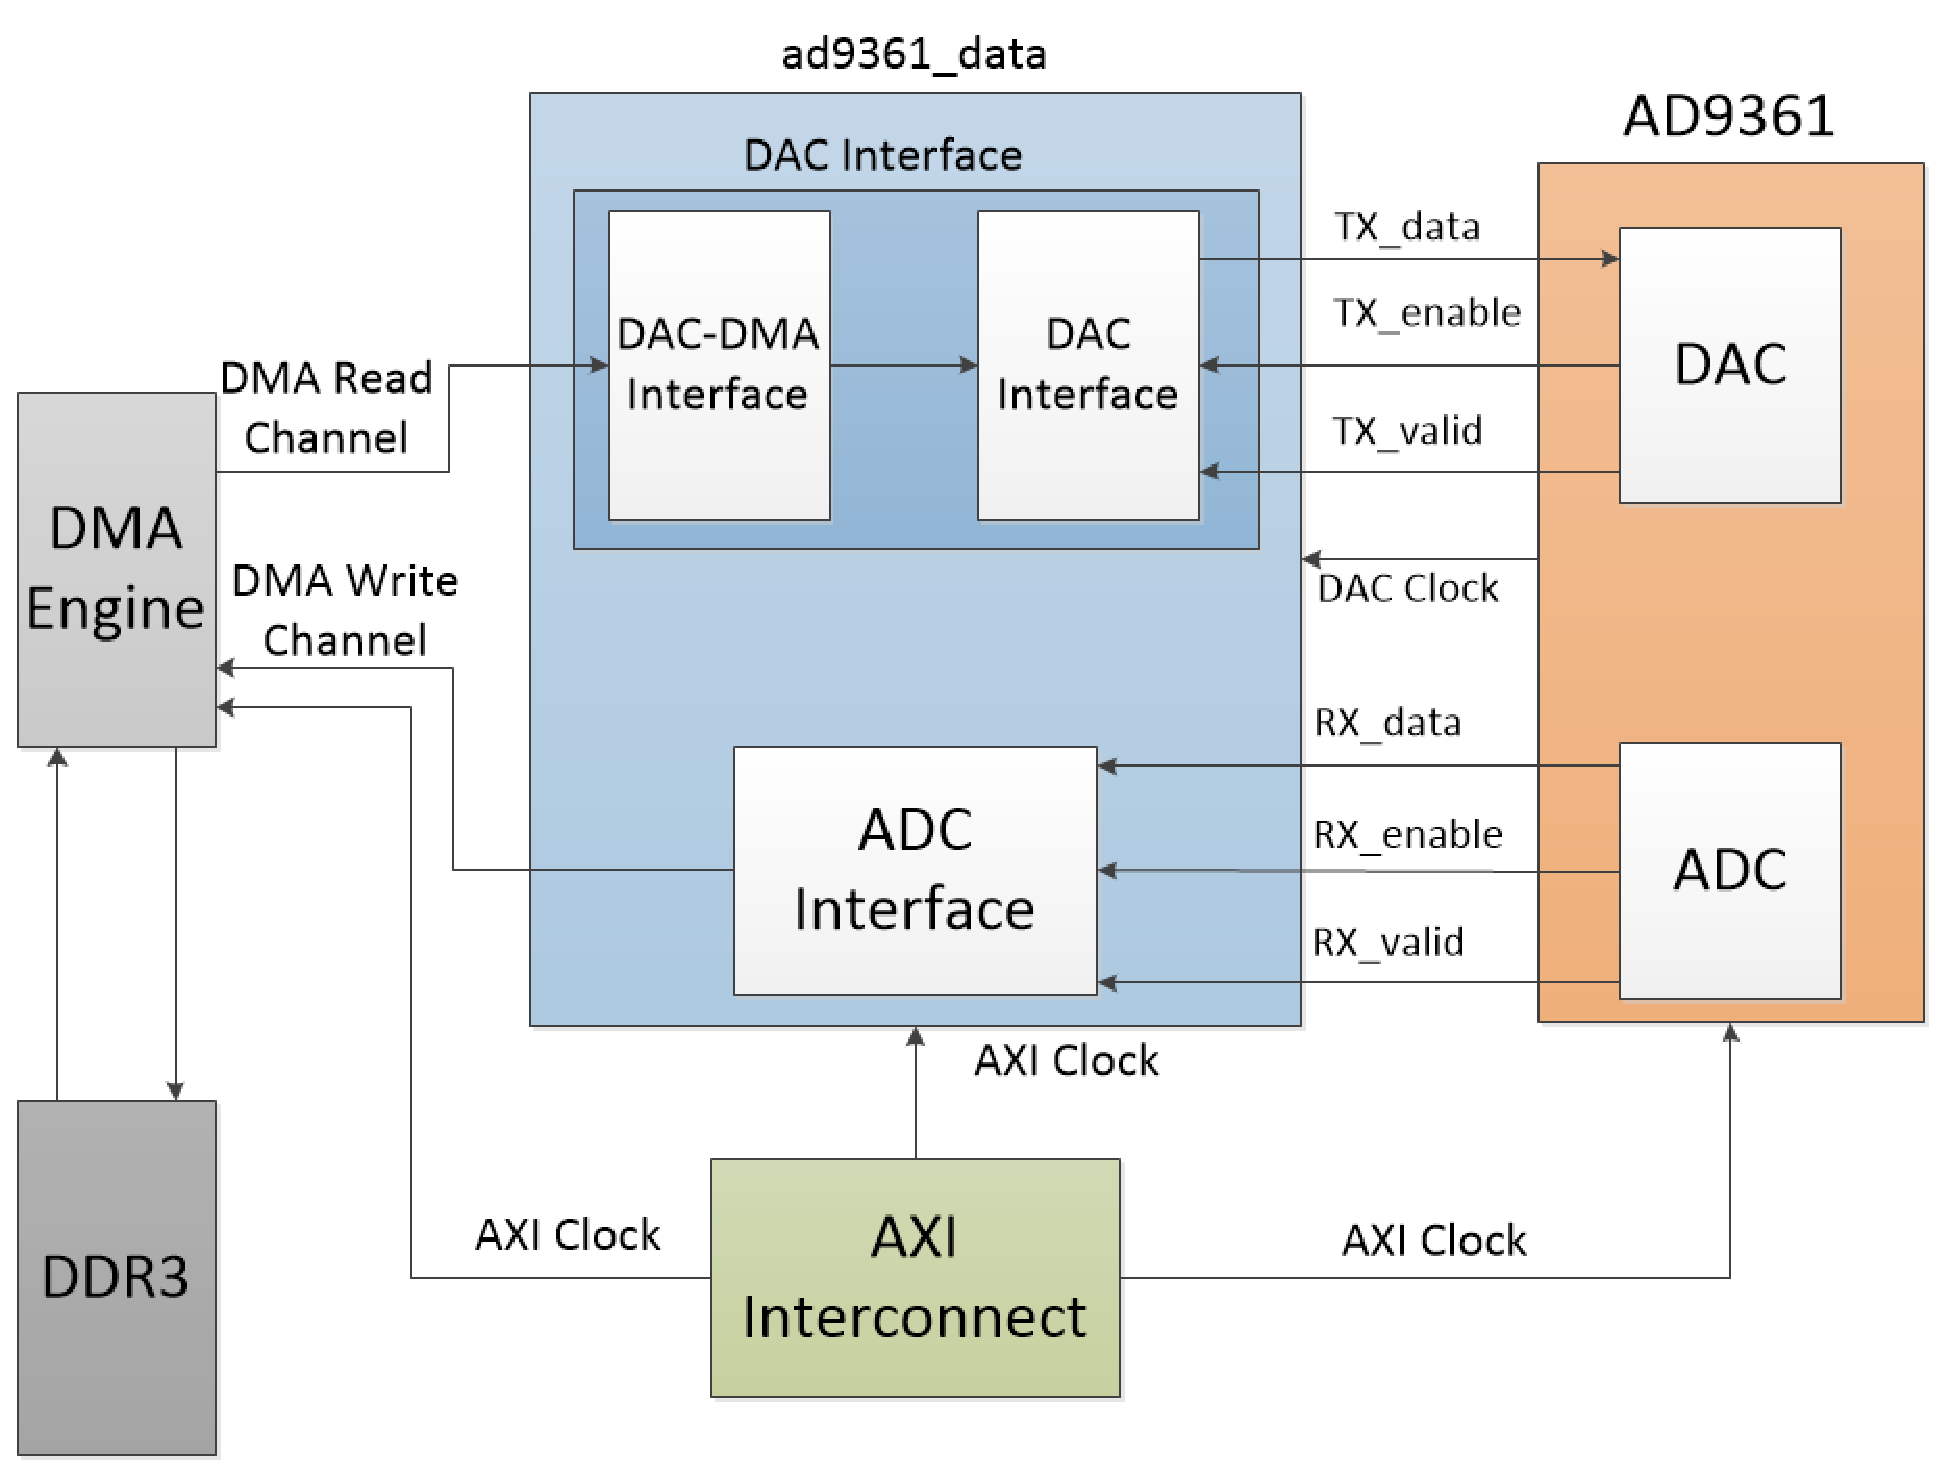
\includegraphics[width=0.85\textwidth]{./figures/data_if}
    \caption{ AD9361 data interface block diagram.
    \label{fig:databd}}
\end{figure}

\subsubsection{Transmitting Interface (Tx)}

The receiving interface itself is divided in two main blocks, one block being
the \emph{DAC-DMA interface} and the other is the DAC interface. The two blocks
are illustrated in Figure \ref{fig:dataiftx}. The DAC-DMA interface controls the
memory reading channel of the DMA, the objective is to transmit the data stream
from the DMA to the two DAC IQ channels and send back the data flow control
signals to the DMA.This process is accomplished by a de-multiplexer and two
channels of cascaded FIFOs (Axi commuter or AxC in Figure \ref{fig:dataiftx}),
this scheme allows for the 32 bit wide data, that DMA block outputs, to be fed
"simultaneous" to both transmitting (DAC) interfaces, DAC 0 and DAC 1, as can be
seen in Figure \ref{fig:dataiftx}. The behavior of the de-multiplexer block is
controlled by a commuter function that basically makes the de-multiplexer block
to send the same signal in both channels. Another thing worth to mention about
the \emph{DAC-DMA interface} is that all the flow control signals that DAC
outputs go through all the blocks and end up in DMA. This block implements the
propagation of these data flow control signals, in the way that the signals from
the DAC can control DMA reading rate.

The \emph{DAC interface} block is another measure of flow control, since the DMA
works in a higher frequency than the DAC block. The FIFOs in the \emph{DAC
interface} acts as a temporary "memory" to keep the flow continuous and they
also have the role to change the clock domain, such as their writing clock
(DAC-DMA interface) is the master clock of the FPGA AXI clock (100 MHz) and the
read clock (DAC) is the actual DAC sampling clock (30.72 MHz), this role is
illustrated by the dashed line in Figure \ref{fig:dataiftx}.

\begin{figure}[htbp]
    \centering
    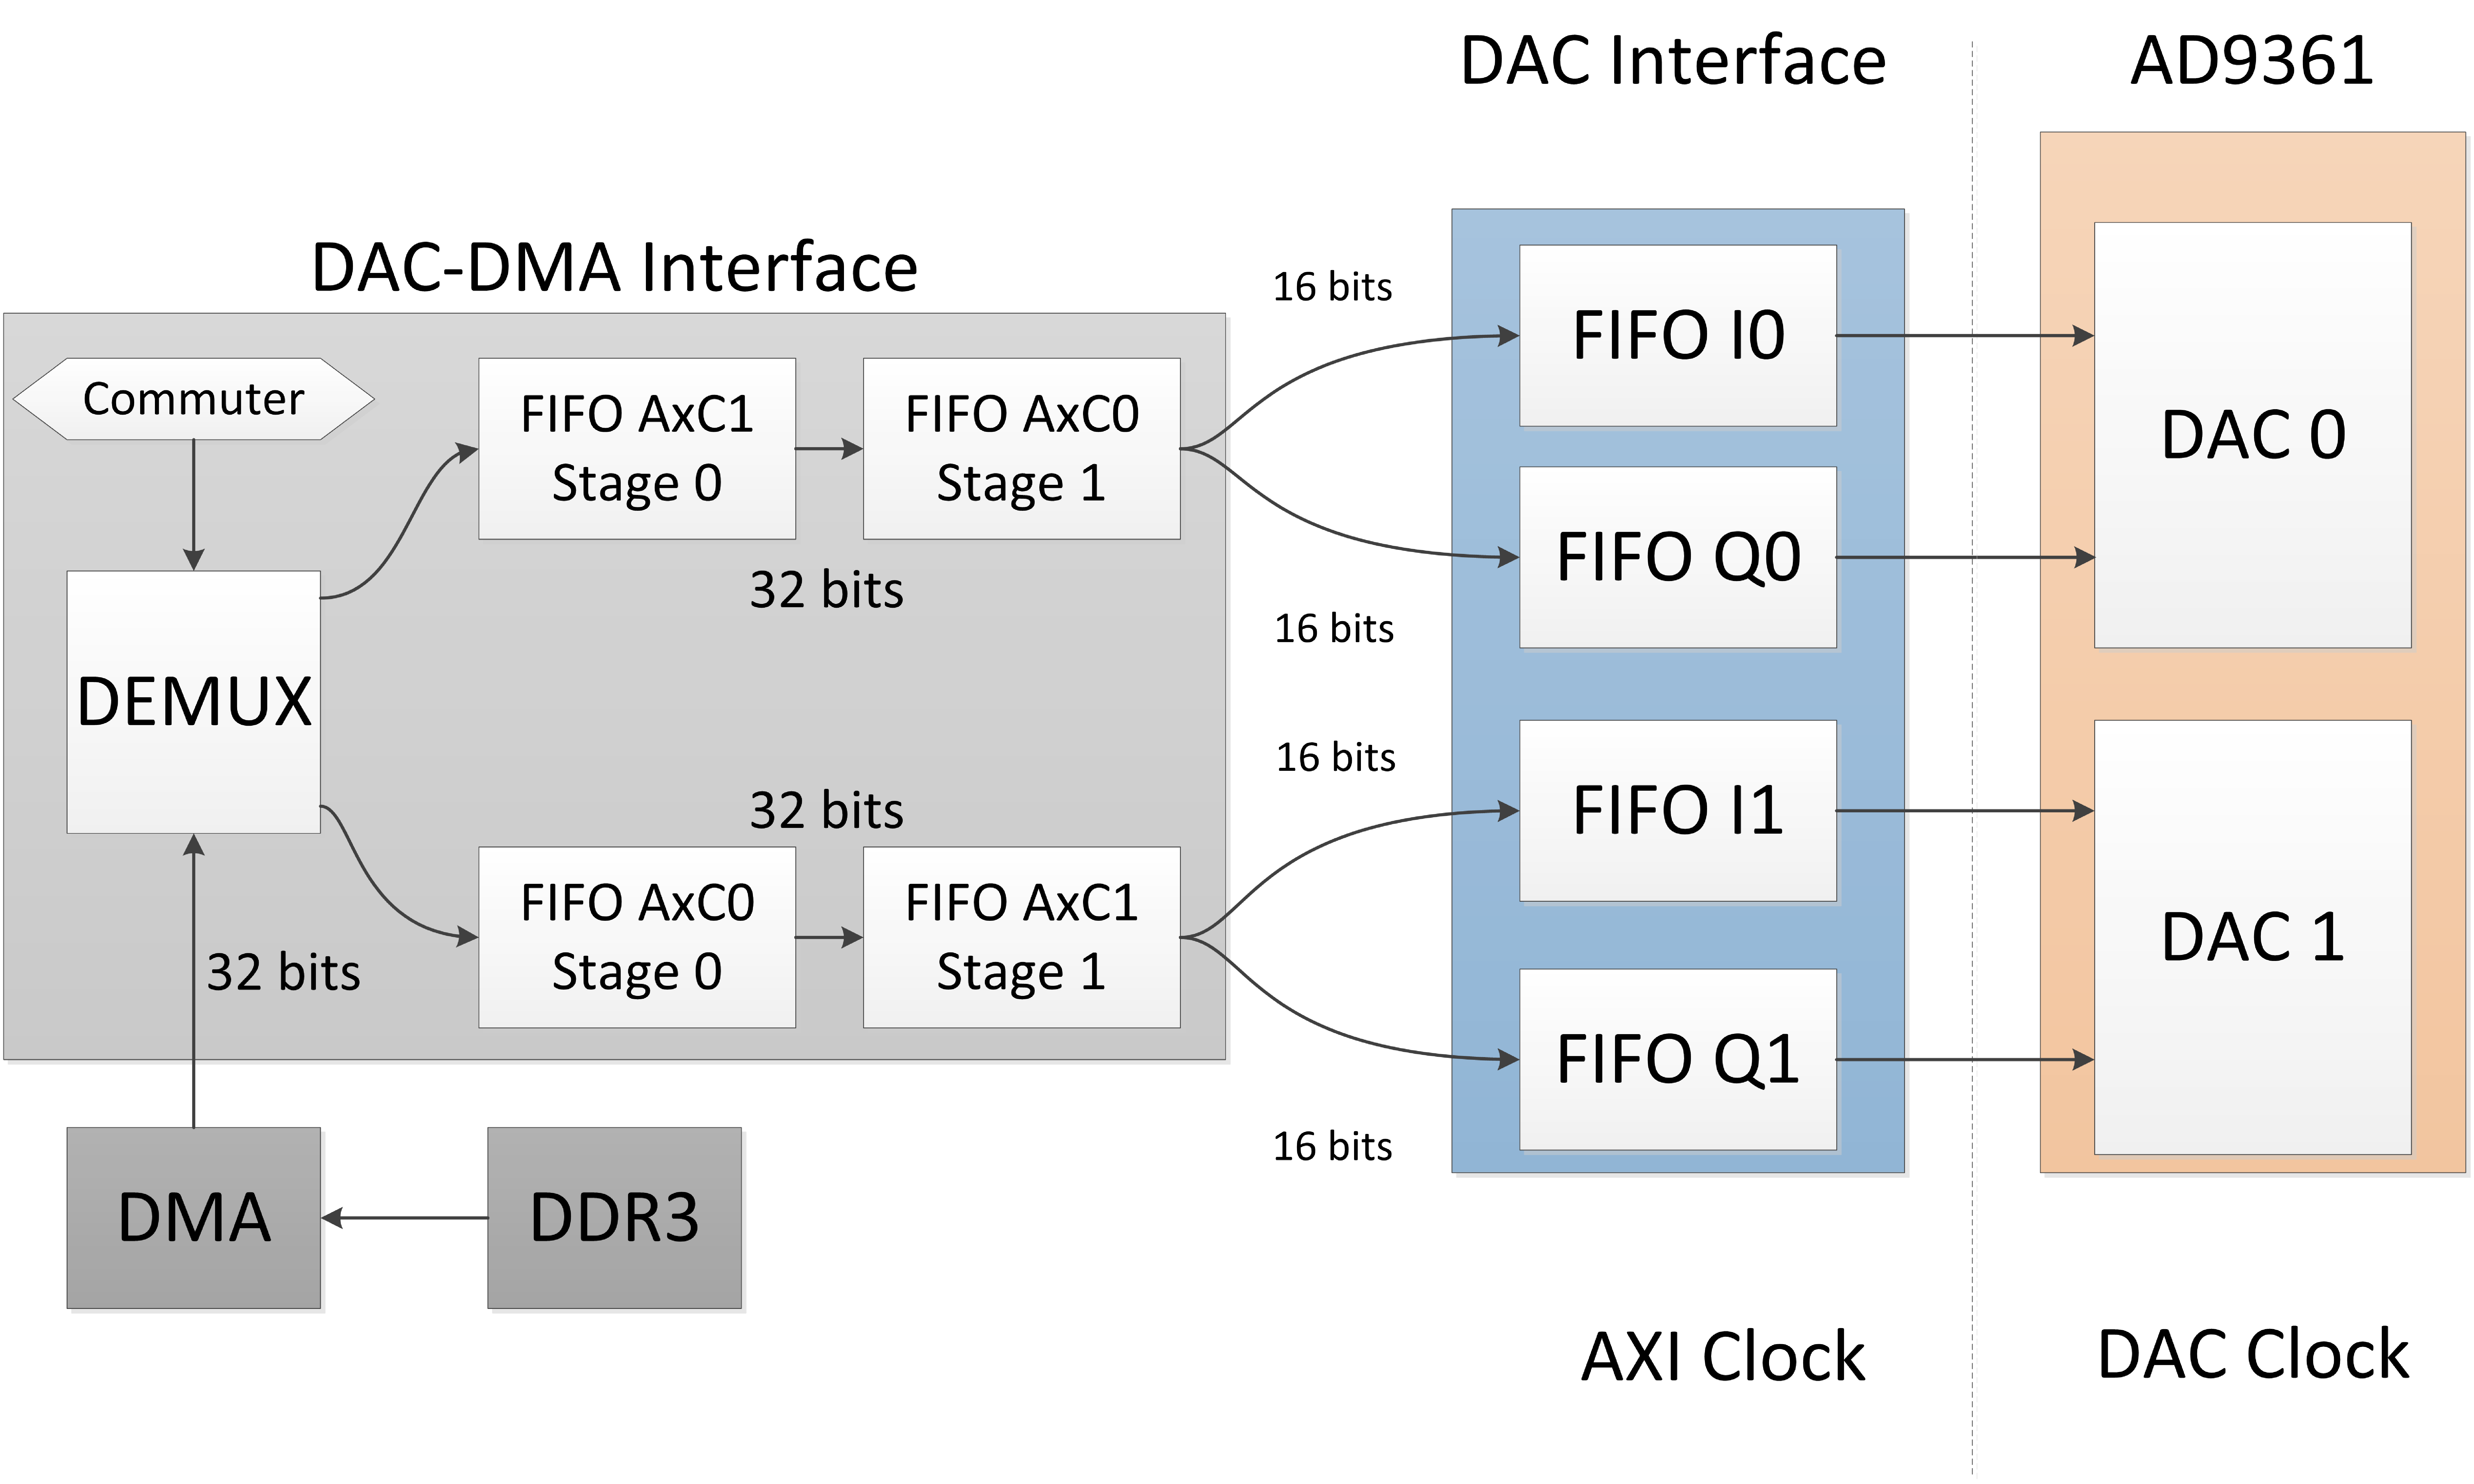
\includegraphics[width=0.9\textwidth]{./figures/txdata_if}
    \caption{ Block diagram of the TX part in the data interface.
    \label{fig:dataiftx}}
\end{figure}

\subsubsection{Receiving Interface (Rx)} %aqui

The receiving interface itself is rather simple in comparison with the
transmitting interface because the speed in which the data is written into the
memory by the DMA is already limited by the DAC clock from the AD9361 interface.
For example, if the ADC is operating at 30.72 MHz, bit rate is 983 mbps
(assuming 32 bits per IQ sample). However, the DMA can operate up to 3.2 Gbps,
so it is capable of much faster inflow of data. In this case, since the DMA
receives data via AXI and the protocol only passes data when data is available,
over flow does not occur. Thus the ADC interface has just to commute both
channels into one (Represented by the "+" in Figure \ref{fig:dataifrx}), feeding
one sample from each ADC channel at a time to the DMA, be able to accomplish
such, there is a state machine to control the FIFO output to the DMA. This state
machine is controlled by the flow control signals outputted by the ADC,
\emph{enables} and \emph{valids} as can be seen in Figure \ref{fig:dataifrx}.
\begin{figure}[htbp]
    \centering
    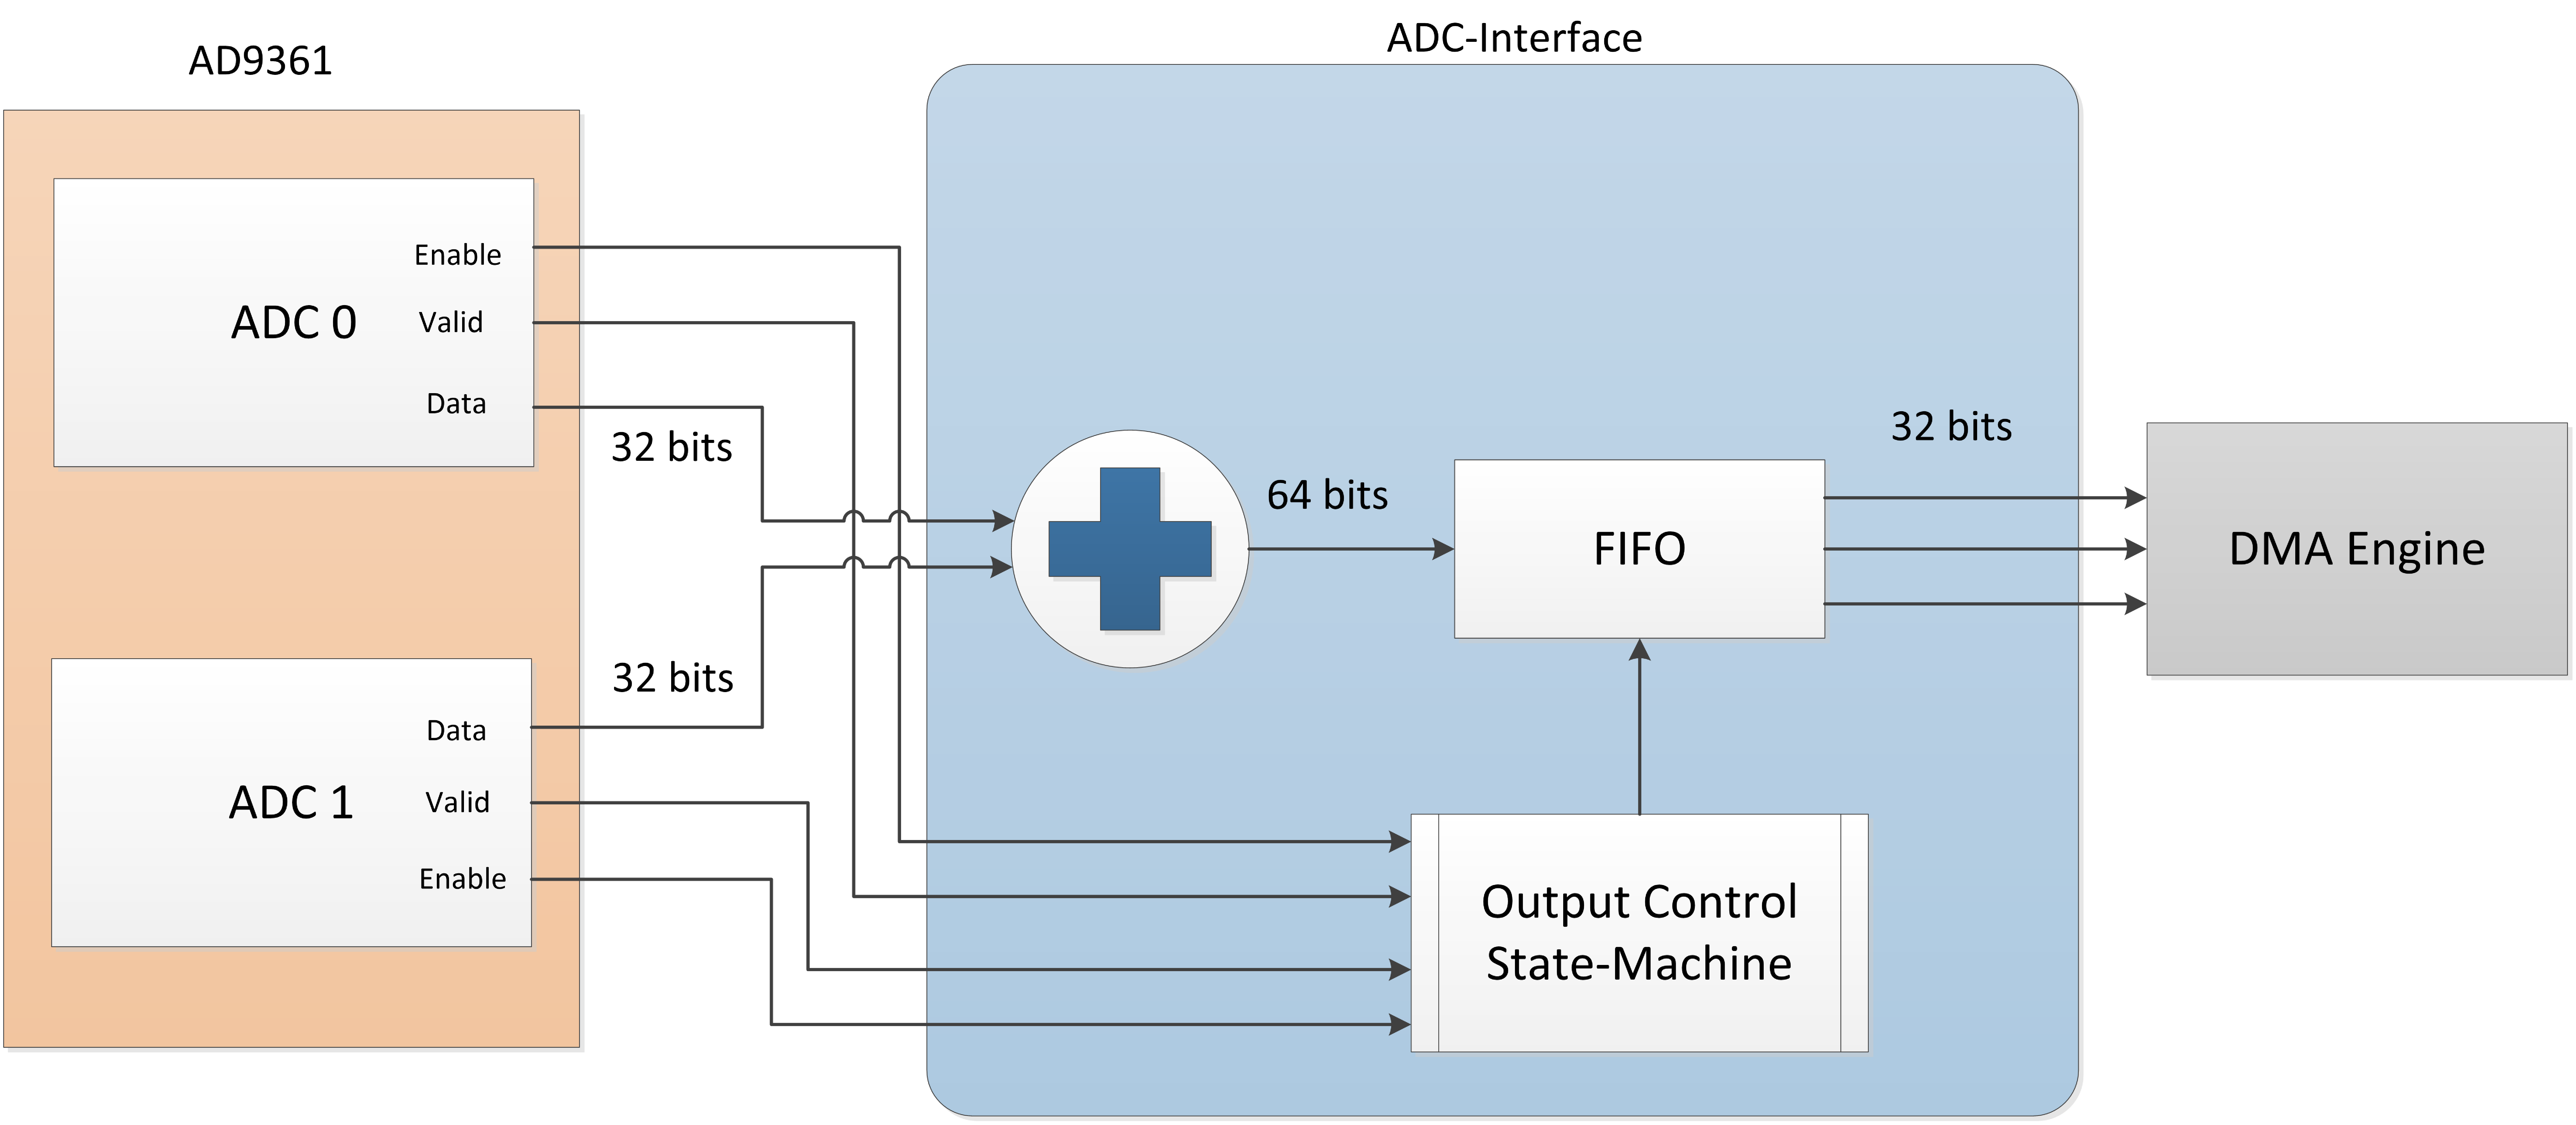
\includegraphics[width=0.95\textwidth]{./figures/rxdata_if}
    \caption{ Block diagram of the RX part in the data interface.
    \label{fig:dataifrx}}
\end{figure}

\section{Driver}
\label{impl:driver}

This setup driver has several parts. It not only initiates the FMComms2 hardware
but also initiates all the systems in the FPGA design, like the interrupt
controller, DMA, SPI and GPIO needed to control and read/write data into the
FMCOMMS2.

The hardware drivers themselves are not extremely complicated nor needed to be
changed too much. Xilinx offers all the basic drivers for the boards, for
example DMA engine, ethernet PHY and interrupt system. The only thing which must
be handled with care is the address space and device ID for each block, knowing
how the IP is configured, or which option he is configured to run is the key to
make a driver work.

Xilinx also packs the design tools with documented examples, one for each
running configuration of the device. There is full support for debugging the
program inside the soft processor Microblaze.

\subsection{AD9361 Driver}

The AD9361 driver is very complex and carries the job of initializing and
configuring the AD9361 chip inside the FMCOMMS2 board. It also initializes the
GPIO and SPI drivers (it can be seen in Figure \ref{fig:ad9361init}), which
functionality are not worth to explain deeply because they are just used for
control and communication and there was no need to modify or to add any
functions to those. The Figure \ref{fig:ad9361init} illustrates all the process
of initiating and configure the AD9361 driver.
The initialization begins in block "AD9361 Initialization" writing in all the
AD9361 registers with the initialization parameters and after this, the driver
initializes all the PLLs and begin to calibrate the analog and digital
interfaces, which is illustrated by the blue part of the Figure
\ref{fig:ad9361init}. With the AD9361 initialization complete it is possible to
change parameters, reconfigure filters and  change oscillators frequency, if any
parameter such as this is changed, the driver must be recalibrate, however it is
done automatically.

In this work there were the need to craft specific filters, set sampling
frequencies and set AGC in order to be able to transmit the waveform stored in
the memory. The order of this process can be seen in the blue part of the Figure
\ref{fig:ad9361init}.

Having every key aspect properly configured the last 2 blocks of the diagram in
Figure \ref{fig:ad9361init} shows that the \emph{DAC initialization} in
\textit{DMA mode} is needed for transmission and \emph{ADC capture} is needed
for reception. The ADC capture function needs to receive also a size (in Kb) of
the capture.

%adicionar diagrama de fluxo da inicialização do ad9361

\begin{figure}[htbp]
    \centering
    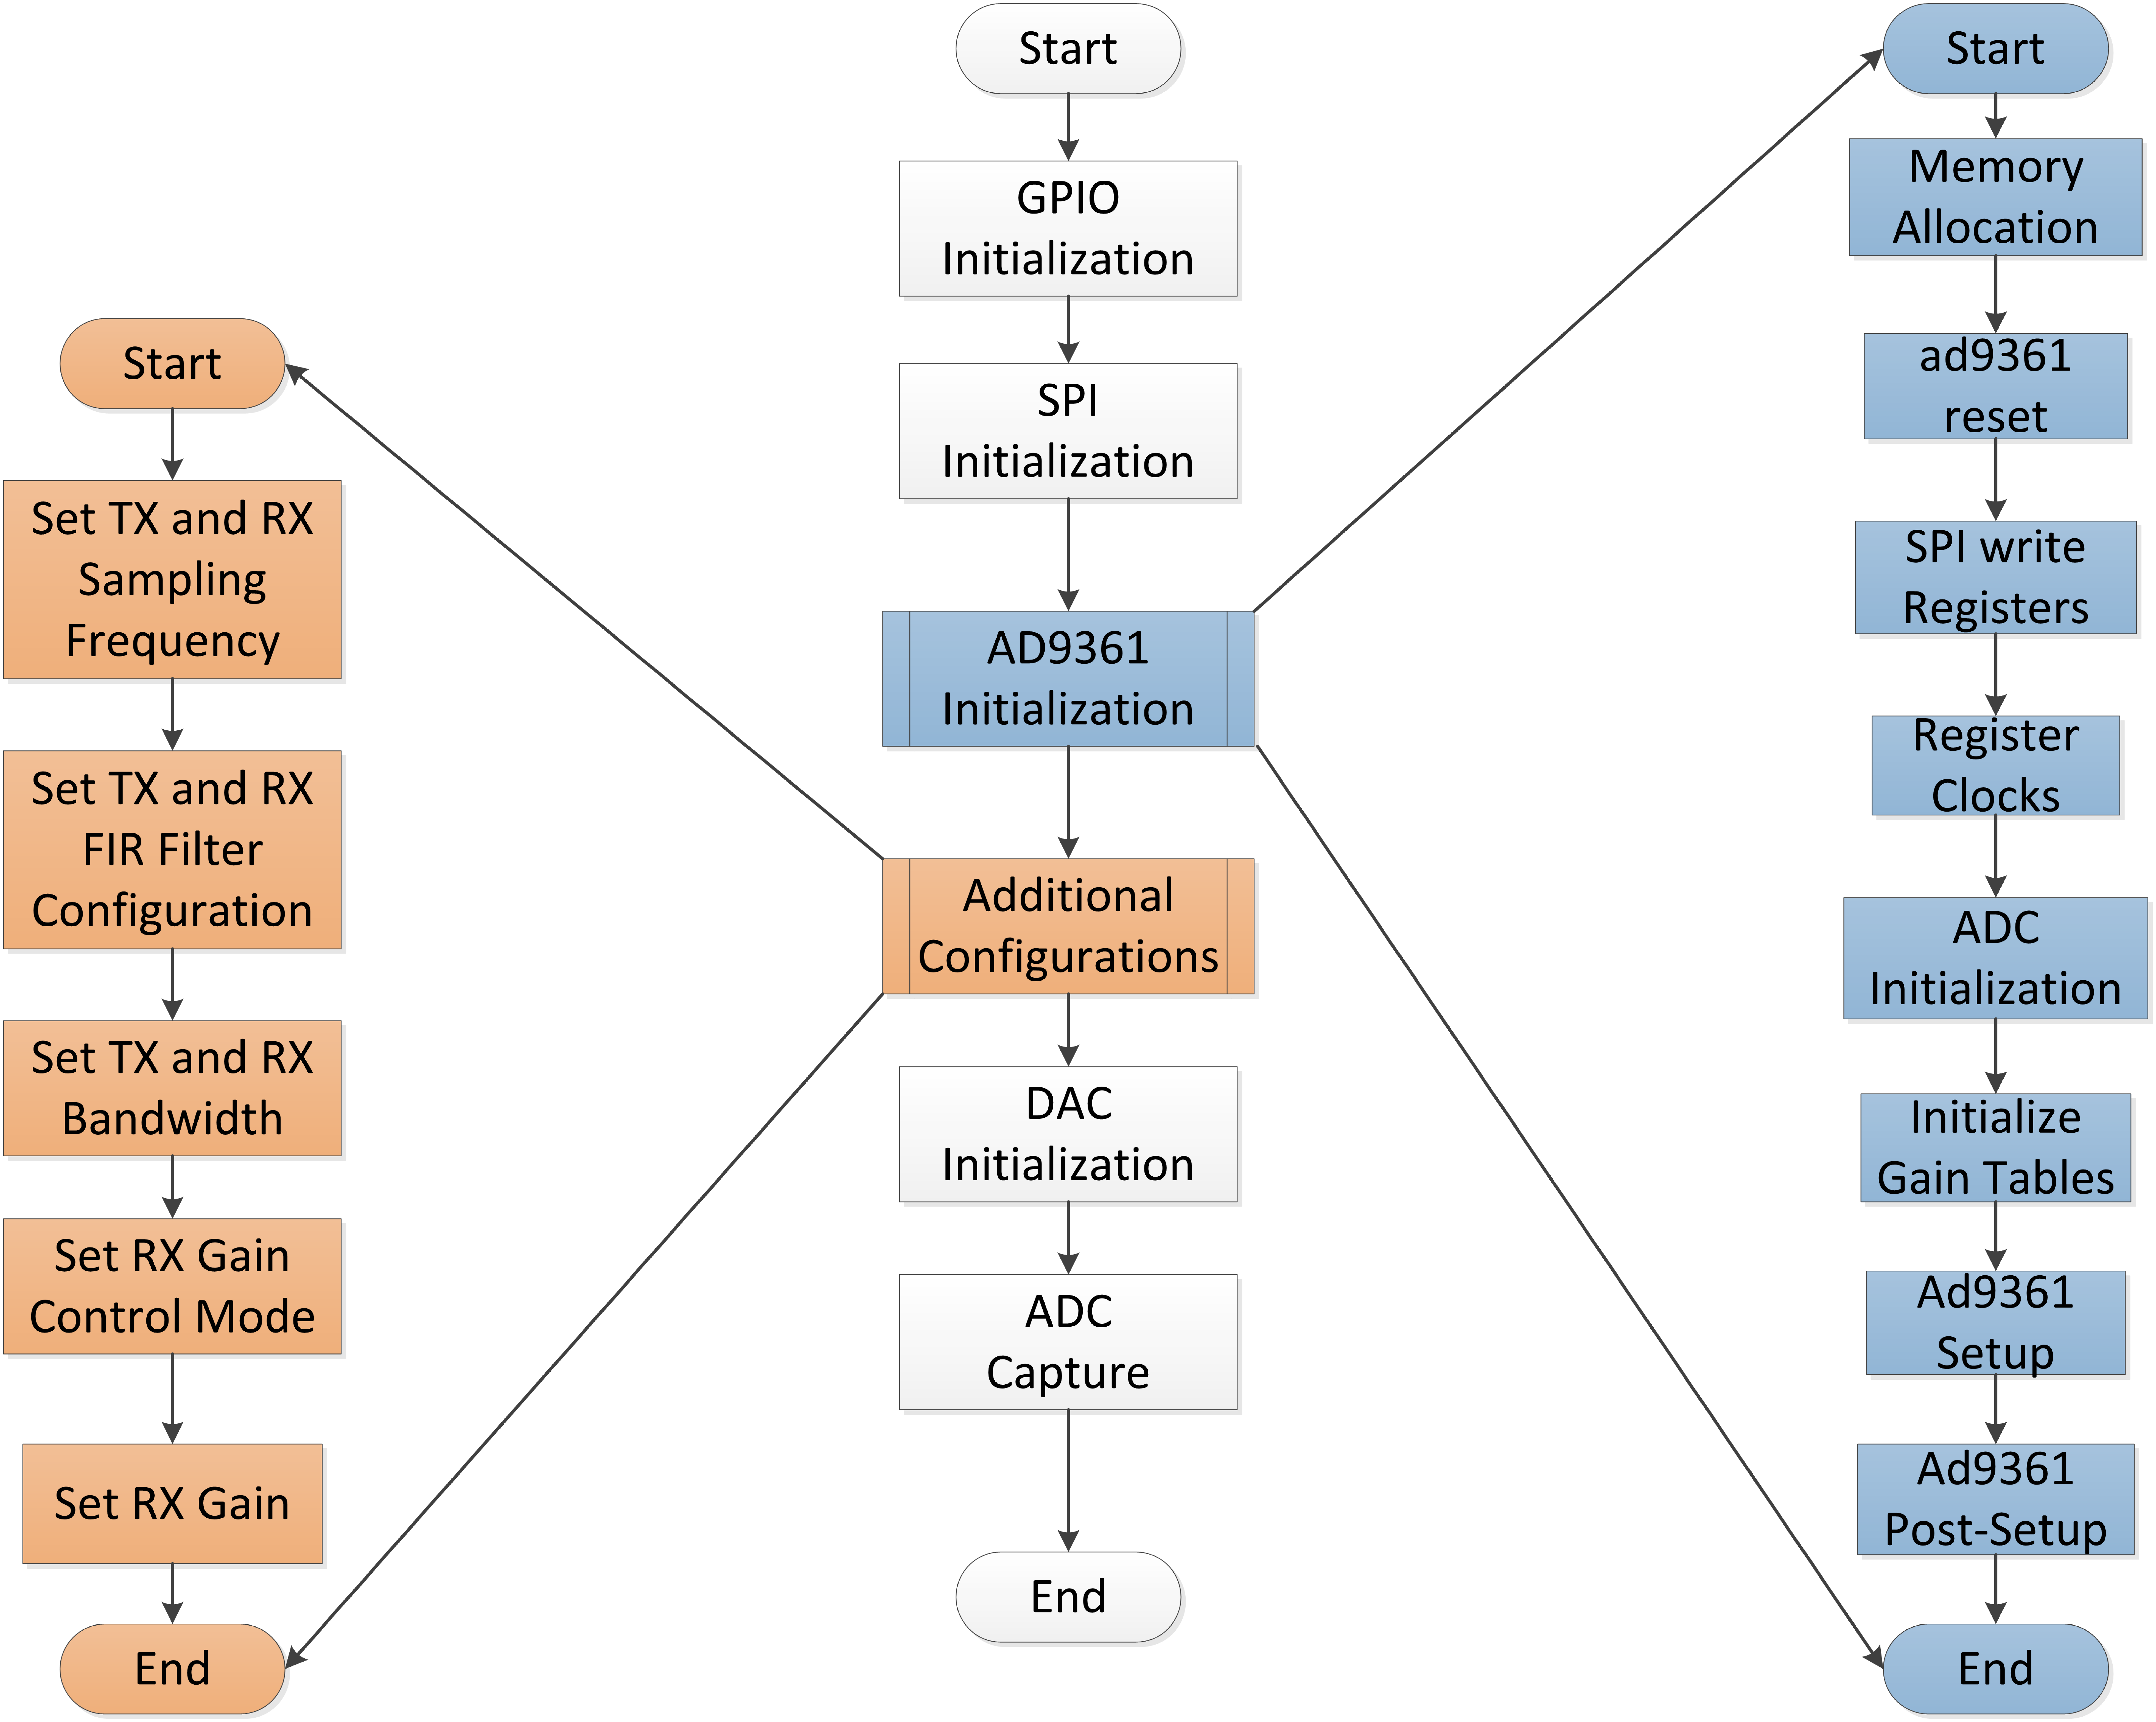
\includegraphics[width=0.75\textwidth]{./figures/ad9361_driver}
    \caption{ AD9361 initialization diagram.
    \label{fig:ad9361init}}
\end{figure}

\subsection{Interrupts and DMA}

Basically FMCOMMS2 utilizes the DMA Engine to read and write in the DDR3 Memory
and the DMA Engine uses interrupts to inform the processor when read and write
data transfers are completed. The DMA has to initialize the configuration, and
then configure the device, which is represented by the block \emph{Interrupt
Controller Initialization} in Figure \ref{fig:intcdmainit}.

After the device is configured, since the DMA is configured in scatter gather
mode, there is the need to allocate the block descriptors (BD) for transmitting
(reading) and receiving (writing), this process is illustrated in the orange
part of the Figure \ref{fig:intcdmainit}. Each block descriptor carries the
initial address of the memory address range to be read, the size of the reading
operation and the address of the next block to read. This allows for the DMA to
read non continuous memory spaces since each descriptor defines an independent
memory region and calls the sequential descriptor (a linked list). After
settting up the BDs the DMA driver has also to setup an interrupt handler for
these blocks, that is a function executed every time an interrupt is asserted.

After all the blocks are processed by the DMA and all the reading is done, the
DMA generates an interrupt to inform the processor that the reading process is
done and in such interrupt routine the cyclic process is implemented,
represented in the blue part of the Figure \ref{fig:intcdmainit}. The process
consists of a loop in the block descriptors, it basically sends DMA back to the
start Block descriptor by the interrupt handler initialized by the DMA driver
and the process of reading the memory runs again and again until the kill signal
is asserted.

In the normal mode, the DMA expects and address an a size, and then it begins
reading or writing in this address until the end of the size and the the DMA
asserts an interrupt and stops. This is not convenient in the prototype
developed in this work, because it was impossible to make measurements in an
oscilloscope or spectrum analyser, the signal would last less than one second,
and doing in cyclic way allows a small number of samples (16 KSamples) to be
transmitted continuously.

\begin{figure}[htbp]
    \centering
    
\includegraphics[width=0.85\textwidth]{./figures/dma_intc_driver}
    \caption{ Interrupts and DMA execution diagram.
    \label{fig:intcdmainit}}
\end{figure}

\section{Applications}
%
This setup was meant to be used in the academic and research and development
environments for such it is extensively documented in this document and in the
source codes in the repository, thus this section aims to be a guideline for
whoever needs to use this work for research or study. Having such role in mind,
all the development was done using \emph{GIT} platform and in this repository
there are all the scripts and instructions to build and replicate this work
\cite{web:gitproject}.

 This project was build in \emph{Vivado Design Tool} version 2015.2.1
\cite{xilinx:vivado} and that is the only software needed to build and
replicate this work. All the development is comprised in \emph{.tcl} scripts,
these scripts are read by \emph{Vivado} and the hardware is built from these
instructions. These is also a section in the project \emph{.tcl} script to copy
the needed files from the directory tree and generate the program with all the
driver initiations.

This setup cannot generate its own waveforms, it has a waveform loaded in a
\emph{.h} file that is loaded by the DMA in cyclic transmission. This waveform
need to be generated in a software like \emph{MATLAB} and the loaded as a
source. The Analog Devices company has already generated some LTE signal samples
which are on their \emph{GIT} repository \cite{web:gitanalogdevlte} and the
instructions are on how to use these tools to generate signals are in
\cite{web:analogmatlabwiki}.
